\synctex=1
%%%%%%%%%%%%%%%%                                ~~~~~~~~~~~~~~~~~~~~~~~~~~~~~~~~~~~~~~~~~~~~~~~~~~
% CONDITIONALS %
%%%%%%%%%%%%%%%%                                ~~~~~~~~~~~~~~~~~~~~~~~~~~~~~~~~~~~~~~~~~~~~~~~~~~

\newif\ifPeerReview\PeerReviewfalse              % Whether to create the PeerReview version or
                                                % Journal version
\newif\ifOnlineColor\OnlineColortrue            % Compile online color version?

\newif\ifFlatArchive\FlatArchivefalse           % Whether archive is flat (messy) or contain 
                                                % subfolders for graphics etc.
\newif\ifFloatAtEnd\FloatAtEndfalse             % Available in PeerReview mode:
                                                % Place floats at end of document?
\newif\ifTODO\TODOtrue                        % Use todo notes?

\newif\ifBuildBibliography\BuildBibliographyfalse  % Whether to include the references.bib file or use inline references.

\ifOnlineColor
   \newcommand\figPostfix{_online}              % Colored images online
\else
   \newcommand\figPostfix{_bw}                  % Black and white in journal
\fi

%%%%%%%%%%%%                                    ~~~~~~~~~~~~~~~~~~~~~~~~~~~~~~~~~~~~~~~~~~~~~~~~~~
% IEEEtran %
%%%%%%%%%%%%                                    ~~~~~~~~~~~~~~~~~~~~~~~~~~~~~~~~~~~~~~~~~~~~~~~~~~

\ifPeerReview
\documentclass[10pt,journal,draftclsnofoot,onecolumn]{IEEEtran}
% \newcommand\CLASSINPUTbaselinestretch{1.66}     % http://theoval.cmp.uea.ac.uk/~nlct/latex/thesis/node17.html
\else
\documentclass[journal]{IEEEtran}
\fi

% \RequirePackage[latin1]{inputenc}%              % Set input encoding (optionally latin1)
% \RequirePackage[T1]{fontenc}%                 % Set font encoding
% \usepackage[norsk]{babel}

% Single column review mode:
%\documentclass[12pt,journal,onecolumn]{IEEEtran}
%\newcommand\CLASSINPUTbaselinestretch{2}
%\RequirePackage{calc}
%\RequirePackage{fp} 
% Left margin = 1 inch + hoffset + oddsidemargin (or evensidemargin)
% Adding the 2cm gutter width to the odd/even side margins:
%\setlength\hoffset{0pt}
%\setlength\oddsidemargin{4cm}       % 4cm margins on the left side
%\addtolength\oddsidemargin{-1in}    % Subtract the initial 1 inch
%\setlength\textwidth{21cm-8cm}    % A4 width (21cm) minus margins on either side

%%%%%%%%%%%%%%%%%%%%%%%%%%%%%%                  ~~~~~~~~~~~~~~~~~~~~~~~~~~~~~~~~~~~~~~~~~~~~~~~~~~
% IEEE ''APPROVED'' PACKAGES %
%%%%%%%%%%%%%%%%%%%%%%%%%%%%%%                  ~~~~~~~~~~~~~~~~~~~~~~~~~~~~~~~~~~~~~~~~~~~~~~~~~~

\usepackage{cite}

\ifCLASSINFOpdf
   \usepackage[dvips]{graphicx}                 % Might not work. Use 'latex' instead of 
   \ifFlatArchive\else                          % 'pdflatex'
   \fi
\else
   \usepackage[dvips]{graphicx}
   \ifFlatArchive\else
   \fi
\fi

\RequirePackage[table,dvipsnames,svgnames]{xcolor}

\usepackage[cmex10]{amsmath}                    % cmex10 option to be IEEE explore compliant
\interdisplaylinepenalty=2500                   % Allows multiline equations to be broken

% \RequirePackage{amssymb}

\RequirePackage{array}

\ifCLASSOPTIONcompsoc
   \usepackage[caption=false,font=normalsize,labelfont=sf,textfont=sf]{subfig}
\else
   \usepackage[caption=false,font=footnotesize]{subfig}
\fi

% \usepackage{caption}
% \usepackage{subcaption}
\usepackage{color}
\usepackage{calc}
\usepackage{fp}

% 
% \ifCLASSOPTIONcaptionsoff                       % IEEE promoted hack to turn off captions from the 
%    \let\MYorigsubfloat\subfloat                 % subfloat package should the captionsoff option
%    \renewcommand{\subfloat}[2][\relax]{\MYorigsubfloat[]{#2}} % be specified.
% \fi

\ifFloatAtEnd
\ifCLASSOPTIONcaptionsoff                       % Places float at the end of the document when the
  \usepackage[nomarkers]{endfloat}              % captionsoff options is specified to IEEEtrans.cls
  \let\MYoriglatexcaption\caption               % (PeerReview mode)
  \renewcommand{\caption}[2][\relax]{\MYoriglatexcaption[#2]{#2}}
\fi
\fi

\usepackage{fixltx2e}                           % Fix some twocolumn float problems

% \usepackage{stfloats}                          % Allows: \begin{figure*}[!b]
                                                % (double column figures on top/bottom)

\usepackage{url}                                % Support for handling and breaking URLs

% NOTE: PDF hyperlink and bookmark features are not required in IEEE
%       papers and their use requires extra complexity and work.
% \newcommand\MYhyperrefoptions{bookmarks=true,bookmarksnumbered=true,
% pdfpagemode={UseOutlines},plainpages=false,pdfpagelabels=true,
% colorlinks=true,linkcolor={black},citecolor={black},urlcolor={black},
% pdftitle={Optimal Window Design for the Low Complexity Adaptive Beamformer in Active Sonar Imaging},
% pdfsubject={},
% pdfauthor={Jo Inge Buskenes},
% pdfkeywords={adaptive beamforming, beamforming, complexity, sonar, active}}%
\ifCLASSINFOpdf
%    \usepackage[\MYhyperrefoptions,pdftex]{hyperref}
   \usepackage[pdftex,
    final,                %Keep hyperlink stuff even when in draft mode
    breaklinks=true,      %Break links when necessary
    linktocpage=true,     %Enable link to page?
    linkcolor=black,  %Colour of links to labels within document
    citecolor=black,      %Colour of links to the biliography
    filecolor=red,        %Colour of links to local files
    pagecolor=black,        %Colour of links to other pages withing document
    urlcolor=Blue,        %Colour of the links to external URLs
    colorlinks=true,      %??
    plainpages=false,     %Store roman/arabic numbering differently to avoid
    bookmarksnumbered ]{hyperref}

\else
   \usepackage[\MYhyperrefoptions,breaklinks=true,dvips]{hyperref}
   \usepackage{breakurl}                        % Allows 'dvips' driver to break links
\fi

%%%%%%%%%%%%%%%%%%%%%%%                         ~~~~~~~~~~~~~~~~~~~~~~~~~~~~~~~~~~~~~~~~~~~~~~~~~~
% ADDITIONAL PACKAGES %       
%%%%%%%%%%%%%%%%%%%%%%%                         ~~~~~~~~~~~~~~~~~~~~~~~~~~~~~~~~~~~~~~~~~~~~~~~~~~

% \ifPeerReview
% \let\OldIncludegraphics{\includegraphics}
% \usepackage{letltxmacro}
% \LetLtxMacro{\OldIncludegrsaphics}{\includegraphics}
% \renewcommand{\includegraphics}[2][]{\OldIncludegraphics[width=\linewidth, #1]{#2}}
% \fi

% % \makeatletter
% % \def\maxwidth{\ifdim\Gin@nat@width>\linewidth\linewidth
% % \else\Gin@nat@width\fi}
% % \makeatother
% % \let\Oldincludegraphics\includegraphics
% % \renewcommand{\includegraphics}[1]{\Oldincludegraphics[width=\maxwidth]{#1}}

% \usepackage[maxfloats=40]{morefloats}
\newcounter{todoidx}
% \setcounter{todoidx}

\ifTODO
   \definecolor{todobackground}{rgb}{0.95,0.95,0.95}
   \setlength\marginparsep{1pt}
   \setlength\marginparwidth{35pt}
   \newlength\marginparwidthsmall
   \setlength\marginparwidthsmall{\marginparwidth}
   \addtolength\marginparwidthsmall{-7pt}
   \newcommand\todo[1]{%
      \addtocounter{todoidx}{1}%
      {\color{Red}\bf(\thetodoidx{})}%%\fbox{\bf\thetodoidx{}}}%
      \marginpar{%
         {\vspace*{-10pt}\color{Red}\fbox{\bf\thetodoidx{}}}\\%
         \fcolorbox{red}{todobackground}{\parbox{\marginparwidthsmall}{\raggedright\scriptsize #1}}}}

   \newcommand\todopar[1]{\fcolorbox{red}{white}{\parbox{0.97\linewidth}{#1}}}
\else
%    \usepackage[disable]{./todonotes} 
   \newcommand\todo[1]{}
\fi

\newenvironment{narrow}[2]{%
\begin{list}{}{%
\setlength{\topsep}{0pt}%
\setlength{\leftmargin}{#1}%
\setlength{\rightmargin}{#2}%
\setlength{\listparindent}{\parindent}%
\setlength{\itemindent}{\parindent}%
\setlength{\parsep}{\parskip}}%
\item[]}{\end{list}}

% \usepackage{float}

\ifOnlineColor
   \definecolor{tabBlue}{HTML}{AACCFF}
\else
   \definecolor{tabBlue}{HTML}{CCCCCC}
\fi

%%%%%%%%%%                                      ~~~~~~~~~~~~~~~~~~~~~~~~~~~~~~~~~~~~~~~~~~~~~~~~~~
% MACROS %       
%%%%%%%%%%                                      ~~~~~~~~~~~~~~~~~~~~~~~~~~~~~~~~~~~~~~~~~~~~~~~~~~

\newcommand\graphicsAI[2][]{%
  \immediate\write18{./bin/laFigure #2 #1}%
  \input{result}}%
  
% \DeclareMathOperator*{\argmin}{\text{arg}\;\text{min}}

\newcommand\Fig[1]{Fig.~\ref{#1}}
\newcommand\eq[1]{(\ref{#1})}

\newcommand\Grey[1]{{\color{Grey}#1}}
\newcommand\Red[1]{{\color{Red}#1}}
\newcommand\Blue[1]{{\color{Blue}#1}}
\newcommand\DarkBlue[1]{{\color{DarkBlue}#1}}
\newcommand\LightBlue[1]{{\color{LightBlue}#1}}
\newcommand\Brown[1]{{\color{Brown}#1}}
\newcommand\Green[1]{{\color{Green}#1}}
\newcommand\SeaGreen[1]{{\color{SeaGreen}#1}}
\newcommand\Yellow[1]{{\color{yellow}#1}}
\newcommand\Orange[1]{{\color{orange}#1}}

\newcommand\nn{\nonumber\\}

\newcommand\nmat[1]{\begin{matrix}#1\end{matrix}}
\newcommand\bmat[1]{\begin{bmatrix}#1\end{bmatrix}}
\newcommand\case[1]{\begin{cases}#1\end{cases}}
\newcommand\textbox[2]{\footnotesize\text{\parbox{#1}{\centering\emph{#2}}}}

\newcommand\rand{\text{rand}}
\newcommand\randn{\text{randn}}
\newcommand\rect{\text{rect}}
\newcommand\sinc{\text{sinc}}
\newcommand\tr{\text{tr}}
\newcommand\adj{\text{adj}}

% \newcommand\max{\text{max}}
\newcommand\argmin[1]{\text{arg}\;\underset{#1}{\text{min}}}

\newcommand\qqquad{\quad\qquad}
\newcommand\qqqquad{\qquad\qquad}

% \renewcommand\l[1]{\left#1}
% \renewcommand\r[1]{\right#1}

% {\text{\parbox{1.5cm}{\centering volume hyper- sphere}}}

%Keyword colouring:
\newcommand\kw[1]{#1}
\newcommand\parm[1]{#1}%\color{Black}#1\color{Black}}

\newcommand\of[1]{\scriptstyle(\parm{#1})\displaystyle}
\newcommand\df[1]{\scriptstyle[\parm{#1}]\displaystyle}
\newcommand\var[3]{#1_\text{#2}\of{#3}}

\newcommand\diag{\text{diag}}

% \raisebox{lift}[extend-above-baseline][extend-below-baseline]{text}
\newcommand\mt[1]{\text{\emph{#1}}} %mt = mathtext
\newcommand\mathnorm{\textstyle}
\newcommand\mathbig[1]{\displaystyle#1\mathnorm}
\newcommand\mathsmall[1]{\scriptstyle#1\mathnorm}
\newcommand\mathtiny[1]{\scriptscriptstyle#1\mathnorm}
\newcommand\sfrac[2]{\scriptstyle\raisebox{0.25pt}[0pt][0pt]{$\frac{#1}{#2}$}\mathnorm}
\newcommand\nfrac[2]{\textstyle\frac{#1}{#2}\displaystyle}

\newcommand\sumu[1]{\sum\limits^{#1}\;}
\newcommand\suml[1]{\sum\limits_{#1}\;}
\newcommand\sumb[2]{\sum\limits_{#1}^{#2}\;}

\newcommand\produ[1]{\prod\limits^{#1}\;}
\newcommand\prodl[1]{\prod\limits_{#1}\;}
\newcommand\prodb[2]{\prod\limits_{#1}^{#2}\;}

\newcommand\defeq{\overset{\underset{\mathrm{def}}{}}{=}}

%Math macros:
\newcommand\T{^{\scriptscriptstyle T}}
\renewcommand\H{^{\scriptscriptstyle H}}

\renewcommand\vec[1]{\boldsymbol{#1}}
\newcommand\mat[1]{\boldsymbol{#1}}

\newcommand\Om{O_\text{m}}
\newcommand\Oa{O_\text{a}}
\newcommand\Nl{N_\text{l}}
\newcommand\Nk{N_\text{k}}
\newcommand\1{\vec 1}
\newcommand\I{\mat I}
\renewcommand*\a{\vec a}
\newcommand*\f{\vec f}
\renewcommand*\i{\vec i}
\renewcommand*\k{\vec k}
\newcommand*\n{\vec n}
\newcommand*\p{\vec p}
\newcommand*\s{\vec s}
\newcommand*\w{\vec w}
\newcommand*\x{\vec x}
\newcommand*\y{\vec y}

\newcommand*\A{\mat A}
\newcommand*\B{\mat B}
\newcommand*\C{\mat C}
\newcommand*\E{\mat E}
\renewcommand*\P{\mat P}
\newcommand*\eP{\mat{\hat P}}
\newcommand*\R{\mat R}
\newcommand*\Ri{\R^{-1}}
\newcommand*\eR{\mat{\hat R}}
\newcommand*\eRi{\hat{\mat R}\;\!^{-1}}
\newcommand*\Navg{N_\text{avg}}
\newcommand*\W{\mat W}
\newcommand*\X{\mat X}
\newcommand*\Xd{\X_{\!\Delta}}
\newcommand*\Y{\mat Y}

\renewcommand\argmin{\text{argmin}}


\renewcommand*\P{\mat P}
\newcommand*\V{\mat V}
\newcommand*\M{\mat M}

\renewcommand*\L{\mat \Lambda}
\newcommand*\U{\mat U}
% \renewcommand*\t{\mathtiny{^T}}
% \newcommand*\h{\mathtiny{^H}}
\renewcommand*\t{^T}
\newcommand*\h{^H}

\newcommand\minus{\scalebox{0.75}[1.0]{$-$}}

% \usepackage{tikz}
% \usetikzlibrary{shapes,snakes}
\usepackage{amsmath,amssymb}
% \usepackage{datatool}
% \usepackage{glossaries}

% \newenvironment{outline}
% {\begin{itemize}}
% {\end{itemize}}
% 

\ifPeerReview
\graphicspath{./submission/submit1}
\fi

% \newcommand\multimedia[1]{\textbf{{\color{red}[#1]}}}
\newcommand\multimedia[2]{\href{#1}{#2}}

% \newcommand\mediaPath{gfx/media}
\newcommand\articlePath{http://folk.uio.no/joibu/articles/2015_JOE_LCA}

\newcommand\mediaI{\multimedia{\articlePath/media1.mp4}{Media Movie~1}}
\newcommand\mediaII{\multimedia{\articlePath/media2.mp4}{Media Movie~2}}


\begin{document}

\title{Low-Complexity Adaptive Sonar Imaging}

\author{Jo~Inge~Buskenes, %
        Roy~Edgar~Hansen, %
        Andreas~Austeng%
\IEEEcompsocitemizethanks{\IEEEcompsocthanksitem All authors are with the Department of Informatics, University of Oslo, Norway.}%
\IEEEcompsocitemizethanks{\IEEEcompsocthanksitem R.~E.~Hansen is also with the Norwegian Defense Research Establishment (FFI), Norway.}% <-this % stops a space

% \thanks{Manuscript received April 19, 2005; revised January 11, 2007.}
}

% The paper headers
\markboth{IEEE Journal of Oceanic Engineering}%
{Low Complexity Adaptive Beamformer for Active Sonar Imaging}

% Publishers ID mark:
%\IEEEpubid{0000--0000/00\$00.00~\copyright~2007 IEEE}

% use for special paper notices
%\IEEEspecialpapernotice{(Invited Paper)}

% for Computer Society papers, we must declare the abstract and index terms
% PRIOR to the title within the \IEEEcompsoctitleabstractindextext IEEEtran
% command as these need to go into the title area created by \maketitle.
\IEEEcompsoctitleabstractindextext{%
\begin{abstract}
% 
% \begin{itemize}
% \item Dynamic weights $\Rightarrow$ greater contrast/resolution potential
% \item But:
% \begin{itemize}
% \item Active system $\Rightarrow$ noise and signal correlated $\Rightarrow$ adaptive beamformers no longer robust.
% \item Subarray averaging decorrelate the noise, but in the process we sacrifice resolution.
% \item Computationally complex O($M^3$) due to inversion of a spatial covariance matrix. LCA is only O($MW$). Even if Capon subspace/beamspace versions exist, they remain more complex than the LCA, and is not as ideally suited for implementation of SIMD hardware (GPUs, DSPs, ...).
% \end{itemize}
% \item LCA is inherently robust, is ``parameter free'' once setup with a well designed window set, and can often be implemented with minor modifications to already existing DAS beamformers.
% 
% The angular resolution and contrast in active sonar images depend on the beamformer's ability to receive signals from directions of interest, while suppressing noise and interference emanating from other directions. For sonar arrays, this is achieved by applying weights to the array channels.
% 
% While classical beamformers use predefined windows, adaptive beamformers estimate the optimal window by analytical evaluation of the data. The minimum variance (MV) beamformer, for instance, calculates the set of weights that minimises the variance of the beamformer's output. 
% 
We have studied the low complexity adaptive (LCA) beamformer in active sonar imaging. LCA can be viewed as either a simplification of the minimum variance distortionless response (MVDR) beamformer, or as an adaptive extension to the delay and sum (DAS) beamformer. While both LCA and MVDR attempt to minimize the power of noise and interference in the image, MVDR achieves this by computing optimal array weights from the spatial statistics of the wavefield, while LCA selects the best performing weights out of a predefined set.

To build confidence in the LCA method we show that a robust MVDR implementation typically creates weight sets with shapes spanning between a rectangular and Hamming window function. We let LCA select from a set of Kaiser windows with responses in this span, and add some steered variations of each. We limit the steering to roughly half the \minus{}3\,dB width of the window's amplitude response. Using experimental data from the Kongsberg Maritime HISAS1030 sonar we find that LCA and MVDR produce nearly identical images of large scenes, both being superior to DAS. On point targets LCA is able to double the resolution compared to DAS, or provide half that of MVDR. This performance is achieved with a total of 6 windows; the rectangular window and the Kaiser window with $\beta=5$, in an unsteered version, and versions that are left and right steered to the steering limit. Slightly smoother images are produced if the window count is increased to 15, but past this we observe minimal difference. Finally we show that LCA works just as well if Kaiser windows are substituted with trigonometric ones.

All our observations and experiences point to LCA being very easy to understand and manage. It simply works, and is surprisingly insensitive to the exact type of window function, steering amount, or number of windows. It can be efficiently implemented on parallel hardware, and handles any scene without the need for parameter adjustments.

% An attactive trait of the LCA is its low computational complexity; while the MV beamformer is of O($M^3$), the LCA method is of O($MW$), with $M$ being the number of channels and $W$ the number of windows. We made the LCA perform like the MV method using a well designed set of 30 windows. Hence, unless the array is very small, the proposed method will perform like the MV beamformer or better, and at a fraction of the computational cost.

% \end{itemize}

\end{abstract}

% Keywords (normally not used for peer reviews)
\ifPeerReview\else
\begin{IEEEkeywords}
Beamforming, adaptive beamforming, MVDR, LCA, sonar, active, complexity.
\end{IEEEkeywords}
\fi
}
% \fi

% make the title area
\maketitle

% This command fixes abstract positioning for compsoc articles:
\IEEEdisplaynotcompsoctitleabstractindextext

% (Optional) Add some extra info on cover page of peer review papers:
% \ifCLASSOPTIONpeerreview
% \begin{center} \bfseries EDICS Category: 3-BBND \end{center}
% \fi

% Insert page break and insert second title (peer review mode)
\IEEEpeerreviewmaketitle

\section{Introduction}

% - Nature and scope
% - Past work
% - Methods
% - Brief summary results
% - Brief conclusions 

% The promise is already demonstrated in nature.
% 
% The sonar systems of the future 
% 
% Future sonar systems 
% 
% Great promise in adaptivity
% 
% The greatest untapped 
% 
% The sonars of the future might benefit greatly from adaptivity.
% 
% 
% Future sonars will likely be 

% To make a sonar truly perform better, we need to make it smarter. 
% 
% \IEEEPARstart{F}{uture} sonar systems will merit a much more sophisticated level of adaptivity. 
% 
% \IEEEPARstart{T}{he} next generation sonar systems will be adaptive.
% 
% Making sonars adaptive is the way to take them into the future. 
% 
% The virtue of future sonar systems will be sophisticated adaptivity. 
% 
% Intelligent
% 
% Reactive
% 
% Observe, process, adapt, act. 
% 
% Adaptivity - sense, process, respond
% 
% Faster, smarter
% 
% The best sonars in nature are adaptive. 
% Nature allures us to be this bold because 

\IEEEPARstart{T}{he} best sonars in existence is perhaps found in nature. Bats, for instance, use a high frequency sonar to detect, identify and track prey with amazing precision in caves amongst a myriad of other bats. No man made sonar can currenly match this feat, much due to the challenge of processing and adapting to such a complex environment fast enough. This is why human made sonars have little to no adaptivity on transmit. However, several methods have been investigated to adaptively process the received acustic data. Perhaps the best studied method for reconstructing a sonar image out of such data is the minimum variance distortion-less response (MVDR) beamformer~\cite{Capon1969}. It adapts the sonar array's spatial response to minimize the influence of noise and interference in the final image.

In many cases MVDR can improve the contrast and resolution of active sonar images compared to conventional static methods~\cite{Blomberg2013,Blomberg2012a,Lo2004}. However, while the computational complexity of conventional beamformers are linear with the number of channels, O($M$), MVDR is at O($M^3$). This is because MVDR relies on estimating and inverting a covariance matrix. The estimation step dominates the computation in sonar systems with less than 32 channels, but here the computational complexity can be reduced and the implementation accelerated significantly using graphics computing units (GPUs)~\cite{Buskenes2014}. For larger systems the inversion step dominates. This can be dealt with by approximating the full covariance matrix with a small one using space reduction techniques such as beamspace processing~\cite{Asen2013}, or the closely related principal component analysis (PCA)~\cite{Kim2014}. Another alternative is to assume spatial stationarity to form more easily invertible Toepliz matrices~\cite{Asl2012}. However, the mentioned methods are still relatively slow compared to DAS.

A much faster and simpler alternative to MVDR is the Low Complexity Adaptive (LCA) beamformer. Based on an idea by Vignon~\cite{Vignon2008}, it was first introduced by Synnev\aa{}g \emph{et al}. in clinical medical ultrasound imaging~\cite{Synnevag2011}, who demonstrated its ability to obtain very similar image quality to MVDR in systems with focused transmit beams. LCA applies a set of predefined and static windows, or apodization weights, and selects the one offering the best noise suppression. It relies on the same optimization criterion as MVDR, thus may be considered a version of MVDR with a discrete and static window solution space. Alternatively, it may be viewed as a multi-apodization technique. One such method is described by Stankwitz \emph{et al}. in radar imaging~\cite{Stankwitz1995}, where the best out of 2 or 3 windows is selected. However, LCA differs in that it typically selects from a larger pool of windows and allows phase-steered variations of them. Phase-shifting the windows has the effect of slighly adjusting the angle the array is steered towards. This gives LCA an adaptive freedom that lies somewhere in between that of traditional multi-apodization techniques and MVDR. How similarly LCA performs compared to MVDR depends on how well the predefined windows represent the constrained solution space of MVDR.

% While using weights that span a bigger space gives LCA greater freedom, not The bigger the space the weights span, the greater the adaptive freedom, but only the solutions that are valid in the constrained solution space can make a difference.

% Instead of adaptively computing the weights, it adaptively selects them. 

Synnev\aa{}g \emph{et al}. suggested using a window set comprised of rectangular, Kaiser (or Kaiser-Harris) and inverted Kaiser functions. In total he let LCA choose from 12 unique windows, 6 of which were phase-shifted versions of a fairly wide Kaiser window, and one were rectangular. Synnev\aa{}g's composition of windows was motivated by the desire to use wide windows with maximum sidelobe suppression near the receiver, and narrow windows at greater depths for maximum sensitivity and depth penetration. While he achieved good results, it was not made clear how many windows LCA needs, or how they ideally should be steered. Also, it is not apparent how LCA performs in sonar systems where the transmit beam is unfocused.

In this study we expand our previous work of applying LCA to active sonar imaging~\cite{Buskenes2011}. We use variations of the parametric Kaiser window, but also compare it to the trigonometric window function. We extend Synnev\aa{}g's work by steering all our windows and not just some, and demonstrate how LCA's performance is affected by the type and number of windows included. Our results are obtained using experimental data from the 32 element Kongsberg Maritime HISAS1030 sonar, which operates at 100\,kHz with an \minus{}3\,dB element opening angle of 23$^\circ$. Although this system was designed as a synthetic aperture sonar (SAS) where an image is synthesized from several pings of data, we will only create images out of single pings (sectorscan imaging) in this study.

Our results show that when MVDR is robustified to work in active sonar imaging, it computes weights with spatial amplitude responses that tend to be symmetric and steered within a fraction of their \minus{}3\,dB widths. When letting LCA choose from Kaiser windows with similar responses, we obtain images with improved noise suppression and resolution. The resolution gain is made predictable by limiting the maximum steering to a fraction of the \minus{}3\,dB width of each window's spatial amplitude response. Overall, LCA produces images that are similar to MVDR, but with a resolution in between that of DAS and MVDR. LCA is also inherently robust, easy to implement, and fairly easy to understand.

This article is outlined as follows: In Section \ref{sec:beamforming} we offer a gentle introduction to beamforming. Then we move on to adaptive beamforming and describe the MVDR and LCA methods in \ref{sec:mvdr} and \ref{sec:lca}, respectively. We use LCA with the Kaiser window which we describe in \ref{sec:lca_kaiser_windows}, explain how we steer it in \ref{sec:lca_steering}, and by how much in \ref{sec:lca_steering_bounds}. Finally we add some remarks on using the trigonometric window instead of Kaiser in \ref{sec:lca_trigonometric}, and of of sampling considerations in \ref{sec:lca_oversampling}. Results and discussion are provided in Section \ref{sec:results_discussion}, where we study MVDR's windows to find suitable LCA ones in \ref{sec:results_lca_window_function}, assess the range of window types and steering in \ref{sec:results_window_parameters}, determine the number of windows needed in \ref{sec:results_database_size}, and add a note on computational complexity in \ref{sec:results_complexity}. Finally, Section \ref{sec:conclusion} provides a conclusion.

% This article is outlined as follows: In Section \ref{methods}, we introduce the concept of adaptive beamforming and provide details on the MVDR and LCA method. Then, in \ref{maptogpu}, we investigate the complexity issue, discuss means for reducing arithmetic complexity, and detail an implementation that makes efficient use of the GPU's parallel resources. The final design is assessed in Sections \ref{images_and_benchmarks} and \ref{discussion}, where we provide benchmarks, comparisons with similar CPU implementations, and measures of how efficiently our implementation makes use of the GPU's resources.

% - How much oversampling
% - How many parameters, how great a span.
% 
% - Experiementl data, Holmengraa/cross
% 
% - Note on efficiency.
% 
% 
% From our work with MVDR it 
% 
% 
% Traditionally beamformers were static, but as processors get more powerful so with the emergence of more processing power 


% 
% \section{Methods}
% 
% At heart of the image formation process is a technique called beamforming, which creates a focus point at the pixel of interest. It does this by applying a suitable set of delays and weights to the array elements, such that signals emanating from the pixel location are emphasized constructively, while noise and interference from other directions sum destructively.
% 
% In active sonar array imaging, an acoustic wave is transmitted and the received echoes are usually recorded using an array of sensors. Each of these may be independently delayed and weighted such that signals emanating from directions of interest are added constructively, while noise and interference from other directions add destructively. Additionally, a window may be applied to the sensor channels to further adjust the array's spatial response. This process is known as beamforming.% The process of combining the signals from each sensor is known as beamforming.
% 
% 
% 
% 
% % Traditional beamformers such as Delay-and-Sum (DAS) apply predefined windows to all incoming data. However, due to the non-stationary nature of sonar data, the optimal window for any given time instant will generally differ from the next. This is where adaptive beamformers thrive, because they compute the optimal window coefficients for the data at each time instant. The choice of optimisation criteria is what mainly differentiates the various adaptive beamformers. The Minimum Variance (MV) beamformer, for instance, selects the set of weights that minimizes the beamformer output power for any given time instant~\cite{cap69}.
% 
% 
% \section{Background}
% 
% The MV beamformer computes the window coefficients by estimating and inverting a spatial covariance matrix. For improved estimation accuracy the data is averaged in space or time, or both. In addition, a certain amount of diagonal loading is often added to the covariance matrix before inversion. These actions, while leading to statistical robustness, tend to deteriorate the beamformer's performance. Also, the inversion of the covariance matrix has a computational complexity of O($M^3$), where $M$ is the number of elements. The computational burden makes the MV beamformer for large arrays less attractive, and sometimes even infeasible.
% 
% Based on the proposed method by Synnevåg~\cite{syn11}, we have implemented the LCA beamformer that keeps the minimum variance optimisation criterion but reduces the solution space to a discrete set of predefined windows. This reduces the computational complexity to O($MW$), where $W$ is the number of windows in the set. We use the Kaiser window function because it allows us to design a wide range of windows with different mainlobe widths and sidelobe suppression by adjusting the tradeoff parameter $\beta$~\cite{kai66}. In addition we apply steering to each of the windows and constrain the window design to ensure unit gain in the look direction.
% 
% The following will show that the proposed method performs similarly to or better than the MV method.


\section{Receive Beamforming}\label{sec:beamforming}

A sonar image is formed by estimating source locations and amplitudes. For this purpose a spatial bandpass filter is applied to the backscattered wavefield data. The filter is called an array processor or receive beamformer. The basic principle is to apply delay and weights to the sensor channels before summing them up, chosen such that signals from the location of interest are summed coherently, while other sources sum incoherently.

Assume that the wavefield has been sampled by an $M$ element uniform linear array, and that the signal signature has been removed by a matched filter. Let $x_m[\theta,n]$ be the delayed data from the $m$th channel, where the $\theta$ and $n$ are the azimuth angle and range sample of the focus point, respectively. Each angle $\theta$ will be processed independently, so to simplify notation we will assume the dependence on $\theta$ to be implicit from now on. 

The output $z[n]$ of a beamformer is defined as the weighted sum of all the delayed data samples:
%
\begin{align}
z[n] = \w\H[n]\x[n] = \bmat{w_0[n]\\w_1[n]\\\vdots\\w_{M-1}[n]}^H \bmat{x_0[n]\\x_1[n]\\\vdots\\x_{M-1}[n]},\label{eq:beamformer_output}
\end{align}
%
where $w_m$ is the weight factor assigned to channel $m$. A weight set is commonly called a window, apodization or taper function. When the window is real its response is symmetric. Applying a real window that trails off towards the edges creates a response with lower sidelobe levels and wider mainlobe, which translates into improved noise suppression at the cost of reduced resolution, respectively~\cite{Harris1978}.

Conventional beamformers all have static and usually real weights. The reference method is the delay-and-sum (DAS) beamformer, also know as the backprojection algorithm. It delays each pixel into focus, then applies a suitable window, and finally sums the data. The virtue of DAS is its simplicity, robustness to parameter errors, linear processing of the image and the ease of which it can be implemented in parallel hardware.

Adaptive beamformers are dynamic and seek to adjust the array response to better fit the incoming wavefield. This may be achieved by allowing either the weights or delays to change, or both. Here the weights are usually complex, which allows asymmetric responses. One of the most extensively studied adaptive methods is the minimum variance distortion-less response (MVDR) beamformer.

\section{MVDR}\label{sec:mvdr}

MVDR seeks to minimize the power of noise and interference in the output of the beamformer, under the constraint of unity gain in some desired direction $\phi$~\cite{Capon1969}. With the assumption of zero mean data this takes the form of minimizing output variance: 
%
\begin{align}
\underset{\w[n]}{\argmin}\, E\{\big|z[n]\big|^2\} &= \underset{\w[n]}{\argmin}\, \w[n]\R[n]\w\H[n]\nn
\text{subject to } \w^H[n]\a_\phi &= 1.\label{eq:mvdr_definition}
\end{align}
%
Here $\a_\phi$ is a steering vector for an azimuthal steering angle $\phi$, $E\{\cdot\}$ is the expectation operator, and $\R[n] = E\{\x[n]\x\H[n]\}$ is the spatial covariance matrix for the full array. This is a convex optimization problem with the unique solution:
%
\begin{gather}
\vec w[n] = \frac{\Ri[n]\a_\phi}{\a_\phi\T\Ri[n]\a_\phi}.\label{eq:mvdr_weights}
\end{gather}
The problem lies in estimating and inverting the spatial covariance matrix. We have described the exact steps in~\cite{Buskenes2014}: To avoid signal cancellation we apply spatial averaging by computing a mean covariance matrix from a set of subarrays with length $L$~\cite{Kailath1985}, for true speckle statistics we perform temporal averaging over $N_k = 2K+1$ temporal samples~\cite{Synnevag2009}, and to improve robustness to parameter errors we add {\large$\epsilon$} percent of the total output power to the matrix's diagonal~\cite{Cox1987,Maksym1979}. These steps are also needed to ensure that the covariance matrix is numerically well conditioned and hence invertible.

\begin{figure}[tbp]\centering%
\ifPeerReview%
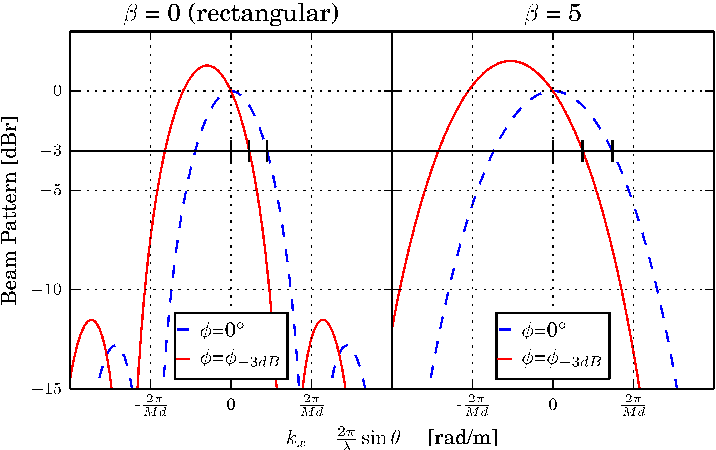
\includegraphics[width=.5\linewidth]{gfx/buske1_online.eps}%
\else%
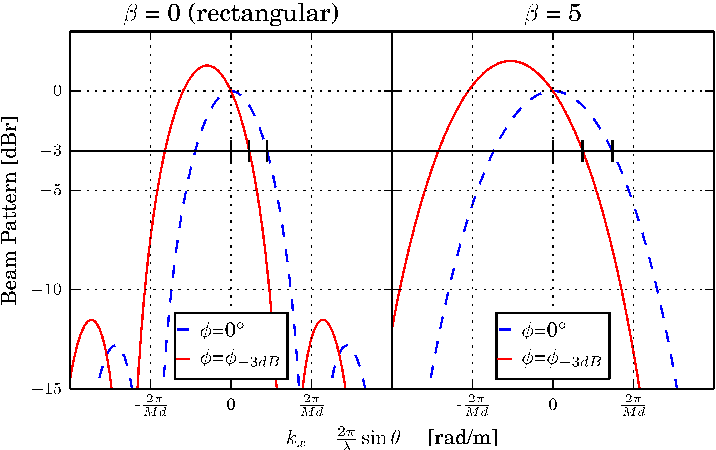
\includegraphics[width=\linewidth]{gfx/buske1_online.eps}%
\fi%
\caption{Each Kaiser window is steered in the interval $\phi\in[0, \phi_{\mathrm{3\,dB}}(\beta)]$. The angle $\phi_{\mathrm{3\,dB}}(\beta)$ is the amount of steering needed for the steered amplitude response to have a \protect\minus{}3\,dB crossing that is exactly half that of the unsteered window. With each window steered this way we expect the resolution gain to remain predictable and independent of $\beta$, and we also effectively constrain the white noise gain of the beamformer.}\label{windows_steering}
\end{figure}

\begin{figure}[tbp]\centering%
\ifPeerReview%
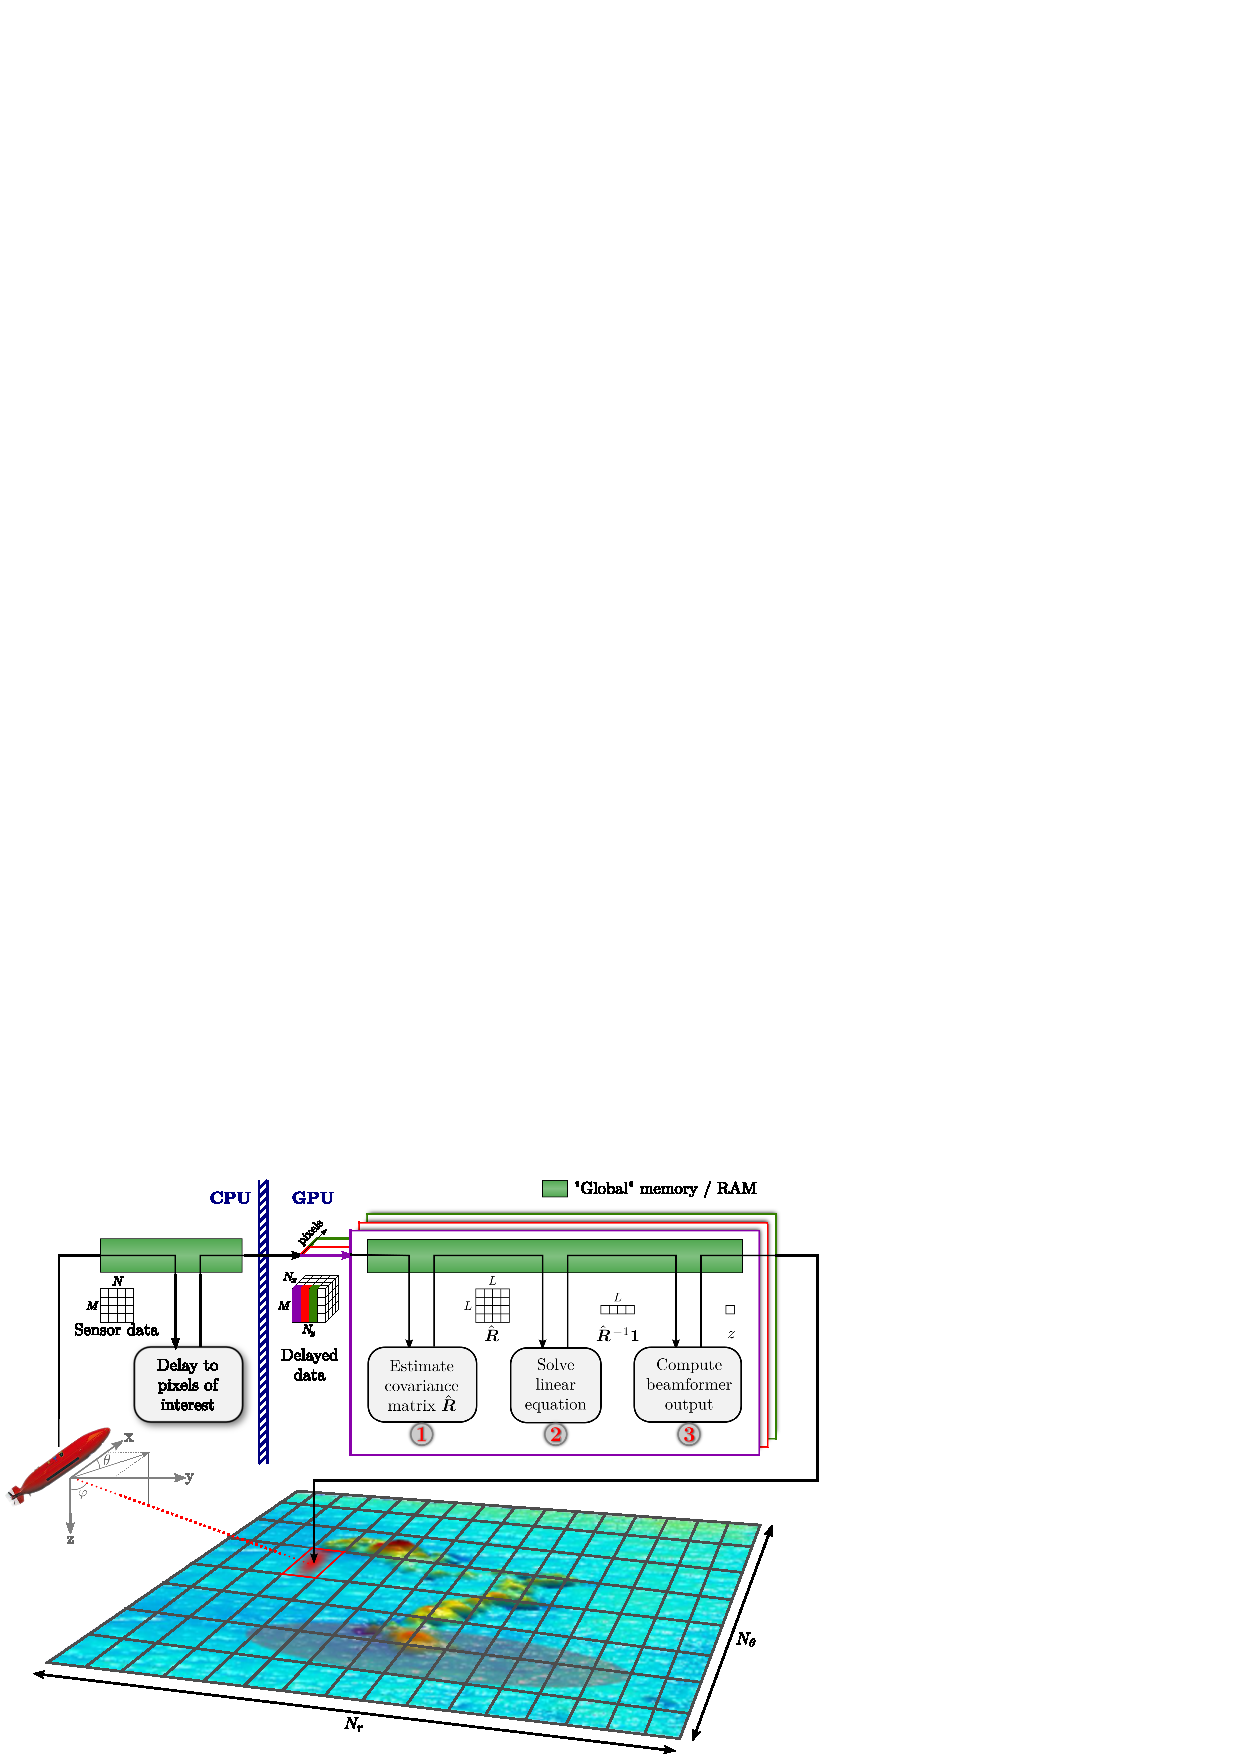
\includegraphics[width=.5\linewidth]{gfx/buske2_online.png}%
\else%
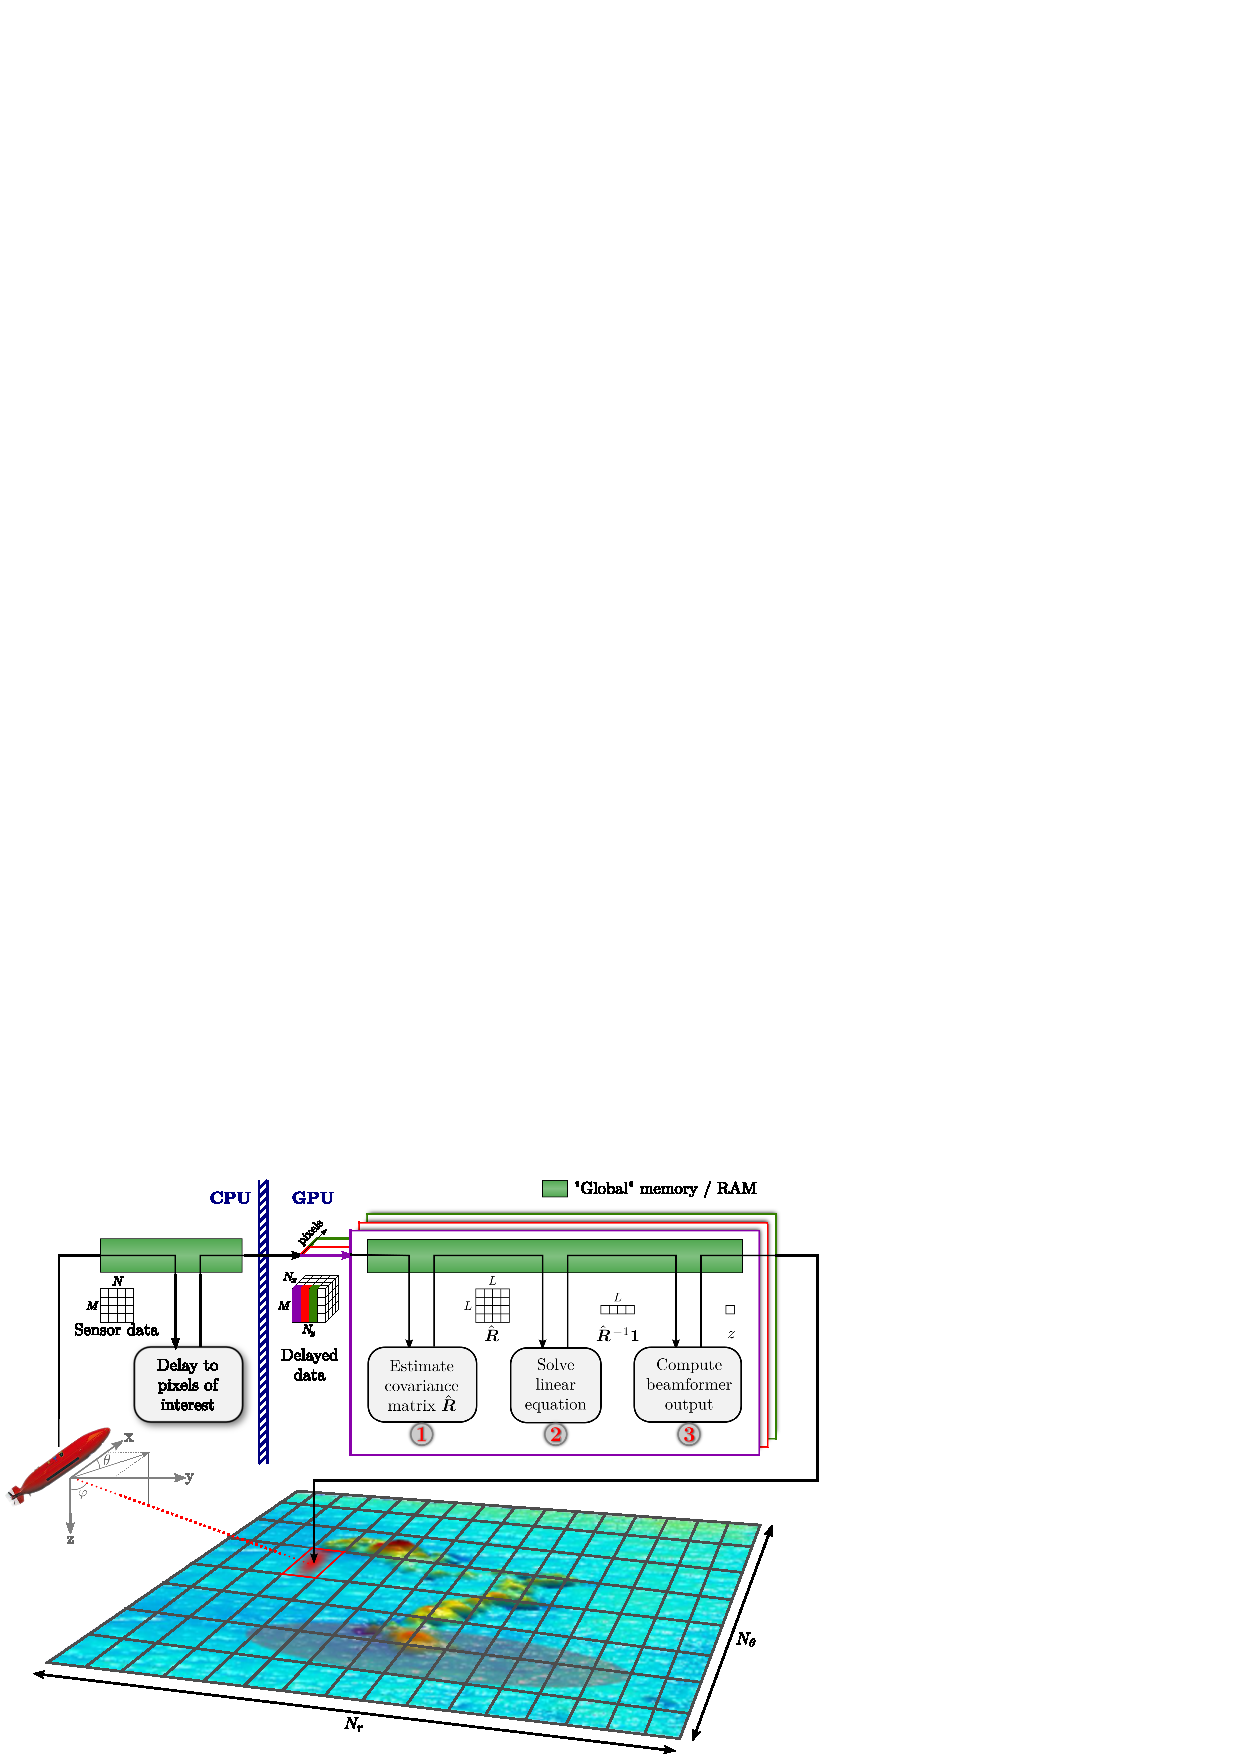
\includegraphics[width=\linewidth]{gfx/buske2_online.png}%
\fi%
\caption{The submerged object used to test beamforming resolution is a 1\,m by 1\,m test cross attached to an anchor with a diameter of approximately 13\,cm. Source image curtesy of Bundeswehr Technical Center for Ships and Naval Weapons, Maritime Technology and Research (WTD 71).}\label{cross}
\end{figure}


\setcounter{topnumber}{1}
\setcounter{dbltopnumber}{1}

\begin{figure*}[t]\centering%
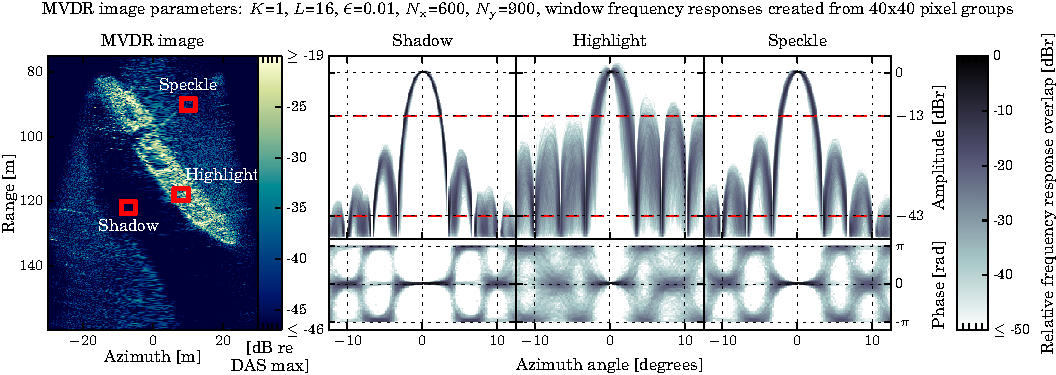
\includegraphics[width=\linewidth]{gfx/buske3_online.pdf}%
\caption{\emph{Determining LCA window type}: MVDR image with typical frequency responses for windows used in various pixel regions.\newline
\emph{Left:}\hfill
\parbox[t]{.95\linewidth}{MVDR sectorscan image of the oiltanker Holmengraa, with 40x40 pixel groups for the shadow, highlight and speckle region of the image indicated with red boxes.}\protect\\\hspace{\textwidth}
\emph{Right:}\hfill
\parbox[t]{.95\linewidth}{MVDR window amplitude and phase responses computed from the 40x40 pixel groups. The responses are overlayed each other and the amount of overlap is colored using a logarithmic scale. The size of the pixel groups were chosen ad-hoc for the histograms to be visually invariant to a shift in position within the same region. Since each pixel is pre-delayed into focus the unsteered responses all have their center at broadside. The dashed red lines at -13\,dB and -43\,dB marks the peak sidelobe levels of an unsteered rectangular and Hamming window, respectively. Note how the responses are more or less symmetric, with very little steering in the shadow, moderate steering in speckle and steering within roughly 3\,dB in highlight. The phase varies most in the highlight region where we see the highest contrast.} }\label{mvdr_selected_windows}
\end{figure*}


\begin{figure*}[t]%
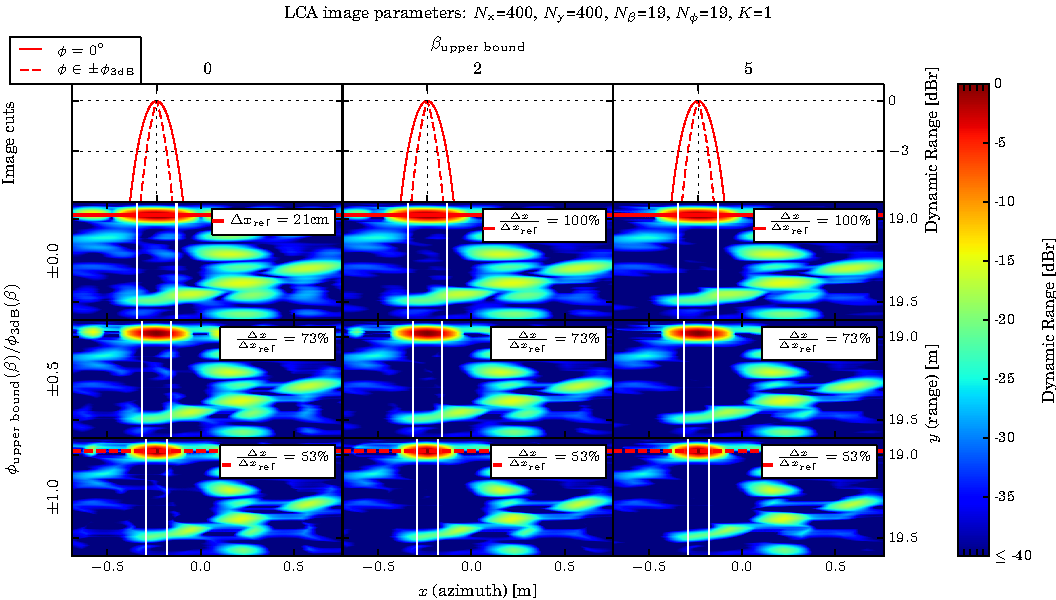
\includegraphics[width=\textwidth]{gfx/buske4_online.pdf}%
\caption{\emph{Determining Kaiser parameter boundaries}: LCA images of the resolution test cross and anchor created with a large window database, but where the upper bounds for $\beta$ and $\phi$ are varied. The upper left image is equal to DAS with a rectangular window. For all images we measure the lateral distance $\Delta x$ between the two \protect\minus{}3\,dB points of the anchor (red object). These are specified relatively to the reference distance  $\Delta x_\text{ref}$ from the upper left DAS image.
\newline
\emph{Upper bound $\beta$:}\hfill
\parbox[t]{.89\linewidth}{Observe that LCA gets better at suppressing sidelobes in the image as we increase the upper bounds for $\beta$. \Fig{mvdr_selected_windows} suggests that MVDR prefers windows with sidelobe levels lower than that of Kaiser with $\beta=2$, but here we observe further improvement going to $\beta=5$.}\newline
\emph{Upper bound $\phi$:}\hfill
\parbox[t]{.89\linewidth}{As we increase the upper bound of the steering $\phi$, we also increase the lateral image resolution. }
}\label{oversampling_mosaic_bounds}
\end{figure*}

% \setcounter{dbltopnumber}{2}

\begin{figure*}[t]\centering
\subfloat[$\beta$-values of the Kaiser window chosen for each image pixel. Note how LCA prefers a narrow response ($\beta=0$) on the anchor, and on other strong sources with little lateral interference. On the sources where lateral interference is present it chooses the widest response with the best sidelobe suppression.]{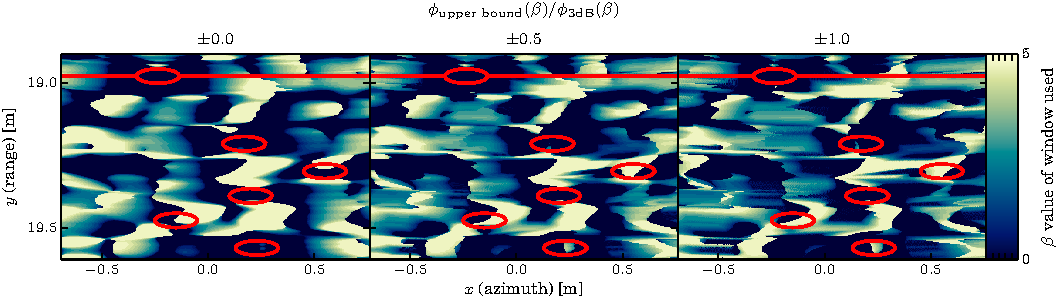
\includegraphics[width=\textwidth]{gfx/buske5a_online.pdf}%%
\label{oversampling_mosaic_bounds_beta}}
\hfil
\subfloat[$\phi$-values of the Kaiser window chosen for each image pixel. On strong sources LCA selects windows that are steered away from the source. This is what improves the FWHM measurement in \Fig{oversampling_mosaic_bounds}.]{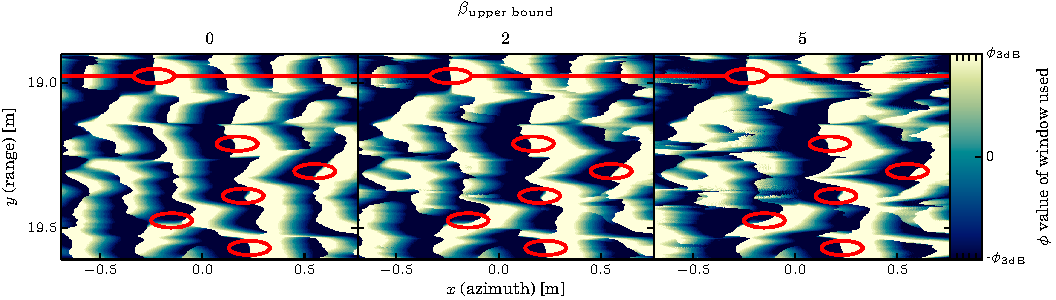
\includegraphics[width=\textwidth]{gfx/buske5b_online.pdf}%
\label{oversampling_mosaic_bounds_phi}}
\caption{Kaiser windows chosen for each pixel in the image of the resolution test cross. The underlying image is the one shown in \Fig{oversampling_mosaic_bounds}, with the same parameters. The location of the anchor, cut line and main scatter locations of the cross is marked in red.}
\label{fig_sim}
\end{figure*}

\begin{figure*}[t]%\centering%
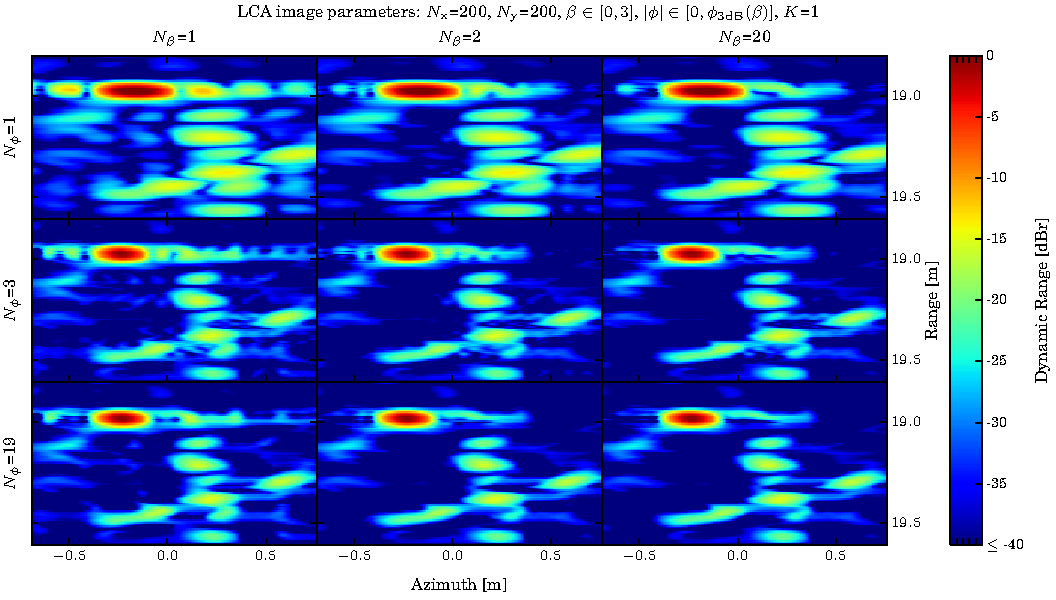
\includegraphics[width=\textwidth]{gfx/buske6_online.pdf}%
\caption{\emph{LCA images using different window database sizes}. The window boundaries are the same. The upper left image is identical to a rectangularly weighted DAS. Observe that finer sampling of the $\beta$-range improves sidelobe suppression but leaves resolution unchanged. Adding more steering-variations improves both sidelobe suppression and resolution. However, using more than  $N_\beta=2$ window types and $N_\phi=3$ steering angles makes minimal difference.}\label{oversampling_mosaic}
\end{figure*}

\begin{figure*}[t]\centering
\subfloat[\emph{Image quality of approximate point scatterers found in the resolution test cross scene}. Two lateral image cuts are shown in the leftmost figures, along with the response of a rectangularly weighted DAS. Note how the FWHM of LCA sits in between that of DAS and MVDR. Also note how LCA is insensitive to the window type; its performance is near identical whether it uses Kasier or trigonometric windows.]{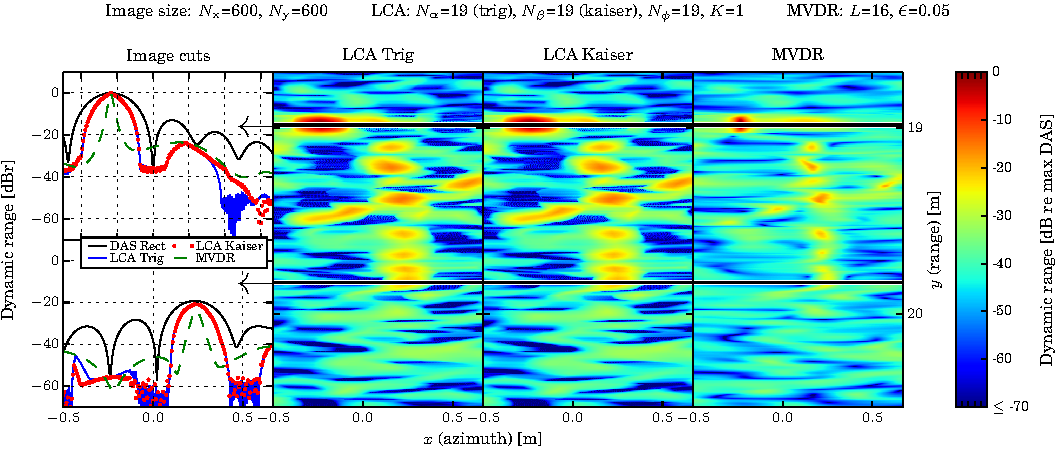
\includegraphics[width=\textwidth]{gfx/buske7a_online.pdf}%
\label{beamformer_comparison_cross}}
\hfil
\subfloat[\emph{Image quality of the full sector Holmengraa scene}. Compared to DAS the adaptive beamformers produce deeper shadows, sharper edges and a higher detail level. The adaptive methods produce nearly identical images.]{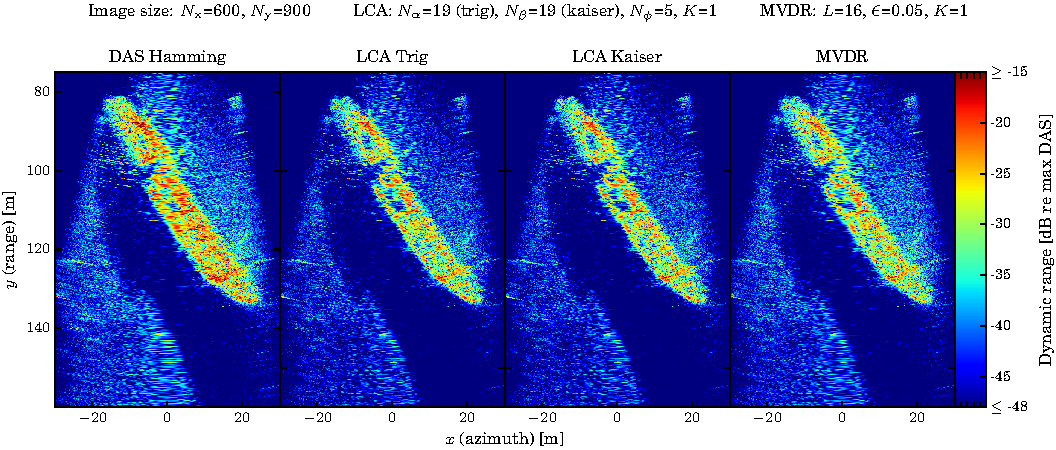
\includegraphics[width=\textwidth]{gfx/buske7b_online.pdf}%%
\label{beamformer_comparison_holmengraa}}
\caption{Comparing image quality of DAS, MVDR and LCA with Kaiser or trigonometric windows.}\label{image_quality}
\end{figure*}


% \begin{figure*}[t]%\centering%
% 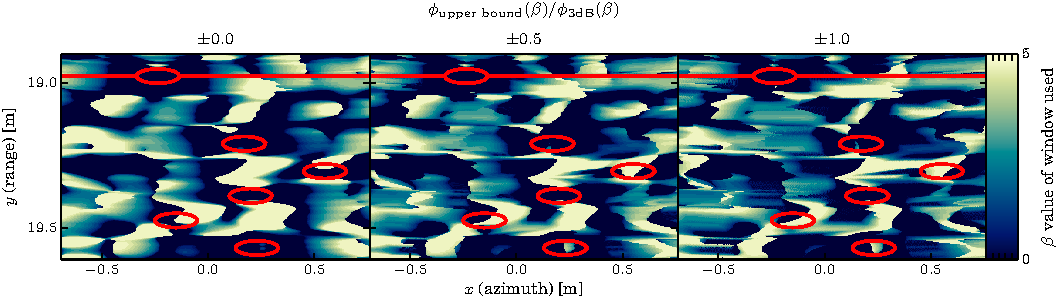
\includegraphics[width=\textwidth]{gfx/oversampling_mosaic_bounds_lca_windows_beta.pdf}%
% \caption{$\beta$-values of the windows LCA selects for each image pixel. The underlying image is the one shown in \Fig{oversampling_mosaic_bounds}, with the same parameters. The location of the anchor and cut line is marked in red. Note how LCA prefers a rectangular window ($\beta=0$) on the anchor.}\label{oversampling_mosaic_bounds_beta}
% \end{figure*} 
% 
% \begin{figure*}[t]%\centering%
% 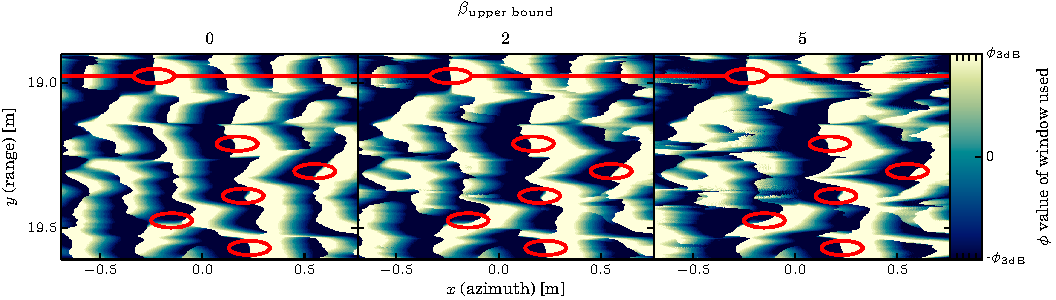
\includegraphics[width=\textwidth]{gfx/oversampling_mosaic_bounds_lca_windows_phi.pdf}%
% \caption{$\beta$-values of the windows LCA selects for each image pixel. The underlying image is the one shown in \Fig{oversampling_mosaic_bounds}, with the same parameters. The location of the anchor and cut line is marked in red. Note how LCA prefers a rectangular window ($\beta=0$) on the anchor.}\label{oversampling_mosaic_bounds_beta}
% \end{figure*} 

% % \setcounter{dbltopnumber}{1

% \begin{figure*}[t]%\centering%
% 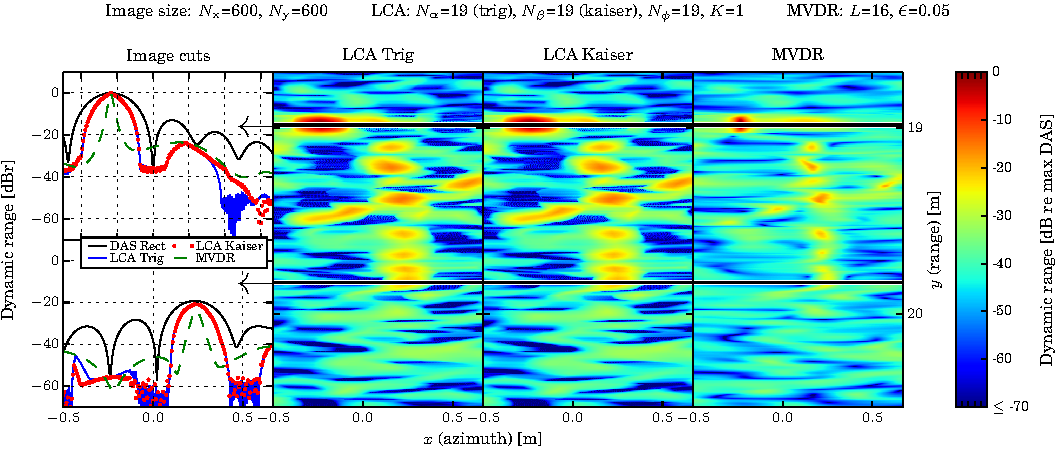
\includegraphics[width=\textwidth]{gfx/beamformer_comparison_cross.pdf}%
% \caption{}\label{beamformer_comparison_cross}
% \end{figure*}
% 
% \begin{figure*}[t]%\centering%
% 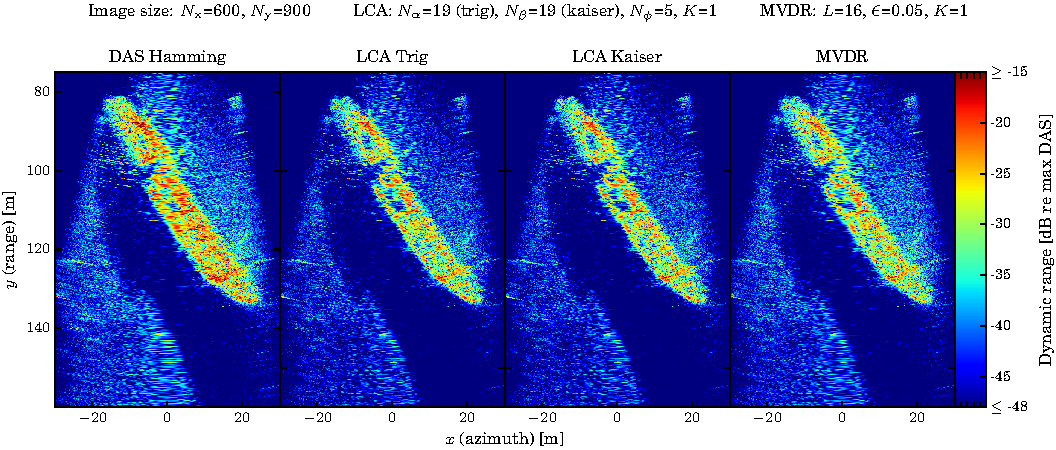
\includegraphics[width=\textwidth]{gfx/beamformer_comparison_holmengraa.pdf}%
% \caption{}\label{beamformer_comparison_holmengraa}
% \end{figure*}


\section{LCA}\label{sec:lca}

A much less complex alternative to MVDR is the low complexity adaptive (LCA) beamformer. It iterates through a set of $P$ windows and selects the window $p$ that best fulfills the minimum variance criterion:
%
\begin{align}
\underset{p}{\argmin}\, E\{\big|z_p[n]\big|^2\} = \underset{p}{\argmin}\, E\big\{\big|\w_{p}\H\x[n]\big|^2\big\}\nn
\qquad\text{subject to}\qquad \w\H\a_\phi = 1.\label{eq:lca_definition}
\end{align}\label{lca_criterion}
%
Note how closely LCA is related to the MVDR definition in \eq{eq:mvdr_definition}. The optimization criterion and constraint is the same, but LCA has a finite and discrete solution space for the weights. As will be demonstrated in Section \ref{sec:results_lca_window_function}, LCA performs similarly to MVDR because a robustified MVDR implementation seems to be constrained to window functions similar to the ones we let LCA choose from.

In practice, we estimate the beamformer output power by computing a sample power average $s_z^2$:
%
\begin{align*}
E\big\{\big|z[n]\big|^2\big\} \approx s_z^2 = \frac{1}{N_k} \sumb{n'=n-K}{n+K} \big| z[n'] \big|^2
\end{align*}
%
which computes the sample power average over $N_k=2K+1$ temporal samples. This is the same temporal averaging method we use for MVDR. In our case the bandwidth of our matched filtered signal is a just few samples long, hence $K=1$ will be used for both MVDR and LCA throughout this work.

If the pixels are correlated laterally, we can include a weighted combination of these to improve the variance estimation:
%
\begin{align}
s_z^2 = \frac{1}{N_x N_k} \sumb{\nmat{\scriptstyle x'=\\[-2mm]\scriptstyle x-X}}{x+X} \sumb{\nmat{\scriptstyle n'=\\[-2mm]\scriptstyle n-K}}{n+K} \omega[x',n']\big| z[x',n'] \big|^2
\end{align}
%
where $N_x = 2X+1$ is the number of azimuth lines to average over, and $\omega[x',n']$ is a normalized 2 dimensional weight function. Since we oversample slightly laterally when we delay each pixel (see Section \ref{sec:lca_oversampling}), we thought the lateral correlation to be sufficient to benefit from this. However, we observed no visual improvement from applying this technique, and decided not to use it.
% 
% \begin{itemize}
% \item \emph{Window function}
% \item \emph{Parameter boundaries}
% \item \emph{Number of windows needed}
% \item \emph{Oversampling need}
% \item \emph{Image quality}
% \end{itemize}


\subsection{Window function: Kaiser}\label{sec:lca_kaiser_windows}

As will be demonstrated in upcoming sections, the LCA beamformer works very well with windows generated from the Kaiser-Bessel function. We will express it in vector form as:
%
\begin{align}
\f_\beta = \bmat{
f_0(\beta) \\
\vdots\\
f_{M-1}(\beta)
}\label{eq:kaiser_window_vector}
\end{align}
%
where
%
\begin{align}
f_m(\beta) = \frac{I_0\left(\pi\beta\sqrt{1-\left(\frac{2m}{M-1}-1\right)^2}\right)}{I_0(\pi\beta)}\label{eq:kaiser_window_element}
\end{align}
%
and $I_0$ is the zeroth order modified Bessel function of the first kind:
%
\begin{align}
I_0(x) = \sumb{a=0}{\infty} \left[ \frac{\left(\frac{x}{2}\right)^a}{a!} \right]^2.\label{eq:modified_bessel_first_kind}
\end{align}
%
The Kaiser-Bessel window is near optimal in the sense of having its peak energy concentration around $\theta=0^\circ$, for a given space-bandwidth product related to the Kaiser parameter $\beta$ as:
%
\begin{align}
\beta = \frac{TB}{2},
\end{align}
%
where $T$ in our case is the spatial extent of the window and $B$ is its bandwidth. Adjusting $\beta$ changes the trade-off between mainlobe width and sidelobe level. When $\beta=0$ the window becomes rectangular, while at large values ($\beta>5$) the window converges to a Gaussian both in time and frequency. This class of windows is generally considered well suited for separating closely spaced sources with amplitudes of a high dynamic range~\cite{Harris1978}, they are easy to make, and they are optimal for any value of $\beta$.


\subsection{Steering}\label{sec:lca_steering}

Adding slightly steered versions of each window to the window database gives LCA greater flexibility in searching for an optimal window. A Kaiser window $\f_\beta$ steered to the azimuth angle $\phi$ can be expressed as 
%
\begin{align}
\w_{\beta,\phi} = \frac{\f_\beta\H\diag{(\a_\phi)}}{\f_\beta\H\a_\phi}\label{eq:steered_window}
\end{align}
%
where diag($\a_\phi$) is a diagonal matrix constructed from the steering vector $\a_\phi$:
%
\begin{align}
\a_\phi = \bmat{
1 \\
e^{-j\frac{2\pi d}{\lambda}\sin(\phi)} \\
\vdots\\
e^{-j\frac{2\pi (M-1)d}{\lambda}\sin(\phi)}
}.\label{eq:steering_vector}
\end{align}
%
Here $d$ is the element spacing, $\lambda$ is the wavelength and $\phi$ is the steering amount. The normalization factor $\f_\beta\H\a_\phi$ is the reciprocal of the window's coherent gain. It ensures unit gain in the direction of interest as required by (\ref{eq:lca_definition}). Since the signal-to-noise ratio is constant for a specific window (same $\beta$-value), this normalization also proportionally increases the incoherent noise gain.

The window database we will construct will contain $N_\beta$ Kaiser windows with unique $\beta$-values, each being steered in $N_\phi$ different directions. This gives us $N_w = N_\beta N_\phi$ unique windows.


\subsection{Steering bounds}\label{sec:lca_steering_bounds}

Each window's spatial response is constrained to unit gain in the look direction. Hence, when it is steered the white noise gain must increase and the the signal-to-noise ratio decrease, as shown in \Fig{windows_steering}. To limit this we place an upper bound to the steering, chosen such that wide windows are allowed to be steered more than narrow ones. We call this upper bound for steering $\phi_{\mathrm{3\,dB}}(\beta)$, and define it as the steering angle needed for the steered amplitude response to have a \minus{}3\,dB crossing that is exactly half that of the unsteered window. The method we devised for finding it is described in Appendix \ref{appendix:steering_angles}. 

Henceforth any steering will be specified relative to this upper bound. With each window steered this way we expect the resolution gain to remain predictable and independent of $\beta$, and we also effectively constrain the white noise gain of the beamformer.

\subsection{Trigonometric windows}\label{sec:lca_trigonometric}

While we focus on using LCA with the Kaiser window function, we will for comparison also test it with the trigonometric window function. Its definition is:
%
\begin{align}
f_m(\alpha) = \alpha - (1-\alpha)\cos\Big(\frac{2\pi m}{M-1}\Big),\label{eq:trig_window_function}
\end{align}
%
where we apply the constraint $\alpha\in[0.5,1]$ to avoid windows with negative coefficients. Steering is applied as in (\ref{eq:steered_window}), and the $\alpha$-value that halves the \minus{}3\,dB distance is found using the method described in Appendix \ref{appendix:steering_angles}. 


\subsection{Oversampling}\label{sec:lca_oversampling}

The ultimate goal of adaptive beamformers is to take the information available in the wavefield and use it to either improve image resolution, sidelobe suppression, or preferably both. This non-linear processing increases the image bandwidth and introduces a need for a sampling rate higher than the Nyquist rate. For MVDR a lateral oversampling factor of 10 compared to the Nyquist rate is often needed to ensure minimal spatial shift-variance in source amplitude~\cite{Asen2014}.

Since LCA operates with the same optimization criterion as MVDR, we will be using approximately a factor 8 lateral oversampling for both beamformers. The images appear more visually pleasing and detailed up to 8. We consider an absolute minimum to be 2, due to the non-linear nature of delaying pixels that isn't strictly in the far field, and of displaying the absolute value of the pixels on a decibel scale. In \mediaI{}\footnote{For media location refer to Appendix \ref{app:source_code}.} we visualize the effect of changing the lateral oversampling factor on a set of LCA images. Upon display the images were all bilinearly upinterpolated to the same size. 
% 
% \todo{Need $M$ in the image sector. Why???}

% Idea to steer within a fraction of the rectangular window's mainlobe. 

% \begin{align}
% d = \frac{\pi\,\theta_\text{open}\,\lambda}{M\,d\,O_s}
% \end{align}


% See section \ref{kaiser_windows}.


% Narrow ones:
% - Best coherent gain, lowest equivalent noise bandwidth, and most sensitive to steering meaning not needing to steer as much for some effect.
% 
% 
% Beamforming:
% - Maximize resolution
% - Minimize noise/error, both coherent and incoherent
% - Minimize signal cancellation
% 
% Gauss: Miminized time-bandwidth product
%   - 
%   
% Rectangular
%   - 
% Dolph-Cheb: Minimize mainlobe width given sidelobe suppression
% Kaiser: For a restricted energy and time duration, maximize energy in the band of frequencies W.
% 
% Adaptive windows perform best in detection of closely separated angles of significantly amplitudes.

% Adaptive beamformers usually compute the window coefficients by estimating and inverting a spatial covariance matrix. There are two inherent problems to this procedure. First, for improved estimation accuracy the data is either averaged in space or time, and the significance of the covariance matrix can be reduced using a regularisation parameter~\cite{Carl Inge}. These are all attempts to constrain the beamformer to ensure the window coefficience are not over-adapted to the data. Second, inverting the covariance matrix has a computational complexity of O($M^3$)~\cite{Carl Inge}. For larger arrays the computational burden becomes significant, and the question arises whether this processing power can be better utilised. 
% 
% 

% 
% This selection is based on observations of the solutions found by the MV beamformer. We obtained good results in our experiments by letting the LCA beamformer select among 5 Kaiser windows with uniformly distributed $\beta$'s in the range $[0.05, 0.5]$ and a rectangular window. Each window was steered in 5 different directions, uniformly distributed within 80\% of the mainlobe width of the rectangular window, which is the most narrow. This adds to a total of 30 windows.
% 
% To make the choice of window less susceptible to pixel value uncertainties, the LCA beamformer was set to apply the most frequently selected window in an 11 pixel range region to the center pixel in that region. In physical terms, this is a region of approximately 20\,cm. The MV beamformer estimated the covariance matrix as described in~\cite{syn07} by averaging over 16 subarrays and 11 range pixels, and applying 3\% diagonal loading.



\section{Results and Discussion}\label{sec:results_discussion}

To test the performance of the MVDR and LCA beamformers, we have processed data acquired by the Kongsberg Maritime HUGIN AUV carrying their 32 element HISAS1030 sonar~\cite{Hansen2011}. It is a high resolution sonar with 1.2\;m array length, 100\;kHz operating frequency, 30\;kHz bandwidth and 23$^\circ$ element \minus{}3\,dB opening angle.

Two different scenes will be studied. One of the 1500 DWT oil tanker wreck Holmengraa lying at a slanted seabed at 77\;m depth outside of Horten, Norway~\cite{holmengraa}. It measures 68\;m by 9\;m and fills most of the highlighted sector. This data was collected by the Norwegian Defense Research Establishment and Kongsberg Maritime. The other scene is of an 1\,m by 1\,m iron resolution test cross, connected to a an anchor with 13\,cm diameter (\Fig{cross}). This data was collected by the Bundeswehr Technical Center for Ships and Naval Weapons, Maritime Technology and Research (WTD 71).

In the image reconstruction we have run MVDR with subarray length $L=16$ and $\text{\large$\epsilon$}=1\%$ diagonal loading. Both MVDR and LCA was run with $K=1$ temporal averaging. This is a fairly aggressive yet stable set of parameters~\cite{Synnevag2009}.

The results will be presented in the following order: In Section \ref{sec:results_lca_window_function} we discuss typical window responses computed by MVDR, and hypothesize that these can be mimicked by Kaiser windows. In Section \ref{sec:results_window_parameters} we determine sensible boundaries for the Kaiser parameter $\beta$ and window steering $\phi$. In Section \ref{sec:results_database_size} we discuss how many window variations are needed for LCA to perform well. 

\subsection{LCA window function}\label{sec:results_lca_window_function}

Assuming that a robust MVDR is the reference method we want LCA to perform similarly to, it seems sensible to create a window database for LCA with spatial responses similar to the ones that MVDR computes. We study this in \Fig{mvdr_selected_windows}, where we present the typical amplitude and phase responses for the windows that MVDR creates in shadow, speckle and highlight regions of the Holmengraa scene.

Observe from \Fig{mvdr_selected_windows} that MVDR seems to prefer symmetric window responses, even if it is free to choose non-symmetric ones. The symmetry is most predominant in shadow and speckle regions, while in highlight the windows are approximately symmetric within the illuminated sector of the seafloor. We have observed this symmetry to be a side-effect of the averaging steps needed to build the sample covariance matrix, which are required for MVDR to operate with very little to no temporal sample support in an active system. The peak sidelobe levels of the MVDR windows are mostly between \minus{}13\,dB and \minus{}43\,dB. This corresponds to that of an unsteered rectangular and Hamming window, or an unsteered Kaiser window with $\beta=0$ and $\beta=2$, respectively.

From this we hypothesize that a good window database LCA can be made using a varied  set of Kaiser windows. If they span a suitable range of $\beta$-values, and some steering variations are applied to each, we should have responses that resemble those in \Fig{mvdr_selected_windows}. The Kaiser window is easy to compute, is fairly insensitive to coefficient inaccuracies, and span shapes from rectangular to Gaussian. It is also optimal in the sense of having its peak power concentration near the steering angle.

Unlike the method described by Synnev\aa{}g~\cite{Synnevag2011} we do not let LCA choose from inverted Kaiser windows. These have a mainlobe width narrower than that of the rectangular window, but at the expense of very poor white noise gain. We have found that these windows hardly ever get used on experimental data, in particular steered versions of them. We can infer the same from \Fig{mvdr_selected_windows} by noting that the maximum sidelobe level rarely exceeds the rectangular window level of \minus{}13\,dB.

\mediaII{}\footnote{For media location refer to Appendix \ref{app:source_code}.} animates how \Fig{mvdr_selected_windows} changes as a function of the MVDR subarray length $L$ and temporal averaging $K$. At $L=1$ the window responses are rectangular in all areas in the image. At $L=2$ we observe window responses with slight amplitude variations in the highlight region, but with the phase being 0$^\circ$ in the illuminated seafloor sector. Already at $L=2$ the MVDR is able to greatly suppress noise. This is a common observation; adding a little flexibility to adapt to the scene has a dramatic effect, but allowing full flexibility is much less significant. The media file also shows that MVDR can be run with subarray sizes $L\in[M/2,5M/8]$, but only with temporal averaging $K=1$ or above.



\subsection{Kaiser parameter $\beta$ and steering $\phi$}\label{sec:results_window_parameters}

To determine a suitable range for the Kaiser parameter $\beta$ and phase steering $\phi$, we constructed large and equally sized window databases containing Kaiser windows with varied upper boundaries for $\beta$ and $\phi$. The lower boundaries were chosen as $\beta=0$ and $\phi=0^\circ$, which includes the rectangularly weighted DAS image. The resulting images are shown in \Fig{oversampling_mosaic_bounds}. In each image we computed the lateral distance $\Delta x$ between the \minus{}3\,dB points of the anchor, with the reference $\Delta x_\text{ref}$ being the rectangularly weighted DAS image. A fourth order polynomial fit was used in this computation. The measure $\Delta x$ is also commonly called the full width half maximum (FWHM). In the case of a imaging a point scatter, it is closely related to the resolution of the system. For a rectangular window, for instance, the system resolution is approximately $\delta x \approx \Delta x/0.89$~\cite{Harris1978}.

The LCA images in \Fig{oversampling_mosaic_bounds} demonstrate the effect of adjusting the upper bound of $\beta$ and $\phi$. As suggested by \Fig{mvdr_selected_windows} we first attempted to use $\beta\in[0,2]$. While this significantly improved sidelobe suppression, a slight further improvement was observed up to $\beta\in[0,5]$. This can likely be explained by the need to compensate for the increased sidelobe levels caused by steering. No noticeable difference were observed for higher values than $\beta=5$. The images also demonstrate that increasing the upper bound for steering $\phi$ improves the resolution of the strong scatterers. For this sonar the Rayleigh resolution is $\delta x\approx0.0125$ radians (0.72$^\circ$), so a point scatterer imaged at 19\,m range with a rectangular DAS would have a lateral $\Delta x\approx0.0125\cdot19\,\text{m}\cdot0.89=21\,\text{cm}$. This is close to the FWHM of the anchor in the DAS image in \Fig{oversampling_mosaic_bounds}, which means that the acoustic fingerprint of the anchor is similar to a point source. This further implies that the anchor reflections are specular and that we view its rounded side. As we increase steering to either 50\% or 100\% of the \minus{}3\,dB width, the FWHM drops to 73\% or 53\% to that of the rectangular window, respectively.

\Fig{oversampling_mosaic_bounds_beta} and \Fig{oversampling_mosaic_bounds_phi} illustrates which $\beta$ and $\phi$ values LCA prefers for different regions in the image of the resolution test cross. Red marker lines are used to pinpoint the cut line, location of the anchor and strong scatters on the cross. Observe that in the anchor region only narrow responses ($\beta=0$) are used, which is the reason for the anchor FWHM being measured to the same value regardless of the upper bound of $\beta$ in \Fig{oversampling_mosaic_bounds}. On other scatterers with strong nearby lateral interference LCA prefers wider windows to suppress the interference. When allowed LCA prefers to steer windows away from the sources, but we never let it exceed the $\phi_\mathrm{3\,dB}(\beta)$ limit. When exceeding this bound we observed oscillation artifacts in the image.


\subsection{Window database size}\label{sec:results_database_size}

So far we have found it reasonable to use Kaiser windows in the range $\beta\in[0,5]$, each steered within the range $|\phi|\in[0,\phi_\mathrm{3\,dB}(\beta)]$. What remains is to determine the number of windows needed. We study this in \Fig{oversampling_mosaic}, where we compare LCA images made from windows databases of different sizes, but with the same parameter boundaries. Included are the results from using a single window ($N_\beta=1$) and steering angle ($N_\phi=1$), which corresponds to an unsteered rectangularly weighted DAS.

Observe that a finer sampling of the $\beta$-range improves sidelobe suppression but leaves resolution unchanged. Adding more steering-variations improves both sidelobe suppression and resolution. We observe major improvement going to $N_\beta=2$ and $N_\phi=3$, but minimal improvement by adding yet more windows.


\subsection{Image quality}\label{sec:results_image_quality}

We compare LCA image quality to that of DAS and MVDR in \Fig{image_quality}. In \Fig{beamformer_comparison_cross} we display the images computed by LCA using Kaiser windows, LCA using trigonometric windows, and MVDR. Two lateral image cuts through all images are presented in the left plot. The images and their corresponding cuts are nearly identical for the LCA version with Kaiser windows and the one with trigonometric windows. Compared to DAS the LCA produces images with an FWHM that lies in between that of DAS and MVDR.

In \Fig{beamformer_comparison_holmengraa} we show full sector images of the Holmengraa wreck. We compare the images produced by a Hamming weighted DAS, by MVDR and by LCA with Kaiser or trigonometric windows. All the adaptive beamformers produce a sharper and less noisy image than DAS, but the difference between LCA and MVDR is minimal. The LCA image produced with Kaiser windows appear identical to that from trigonometric windows.


\subsection{Computational complexity}\label{sec:results_complexity}

The computational complexity of MVDR is generally considered to be of O($M^3$). However, the implementation we are using is optimized so that building the spatial covariance matrix is of O($N_kN_L,L^2$), and inverting it is of O($L^3$). We describe this implementation in \cite{Buskenes2014}, and a beamspace version in \cite{Asen2013}, where we implement it on a graphics processing unit (GPU) for nearly two orders of magnitude speed increase compared to a straightforward C implementation. However, MVDR is not ideal for GPUs due to the complex data dependencies present in the covariance computation, and at best we only managed to utilize 10\% of the GPUs maximum theoretical potential.

In comparison, LCA is of O($M N_\beta N_\phi$), and extremely well suited for GPUs. Each pixel depends on only a small subset of data, and the windows can be precomputed and stored in GPU cache for near immediate access. Furthermore, if we use the trigonometric window function we can solve for the window parameter analytically as described in Appendix \ref{sec:reducing_lca_complexity}. This reduces the complexity to O($M N_\phi$), because the only remaining LCA parameter to create windows for will be the steering angle.

% Furthermore, the algorithm maps well to single-instruction-multiple-data (SIMD) hardware such as graphics processing units (GPUs). We show that even a modest amount of optimisation work has resulted in a factor 10 speed-up of this algorithm when implemented on a GPU as opposed to on a CPU.


% the performance of the LCA beamformer is surprisingly similar regardless of what windows it is allowed to choose from.





% \newcommand\cc[1]{\multicolumn{1}{>{\columncolor{tabBlue}}c}{\bf #1}}
% \begin{table}[!b]\centering%\normalsize
% \begin{tabular}[c]{l r r r@{}  r r r}\hline
% \rowcolor{tabBlue} & \cc{Resolution} & \cc{S} & \cc{$\beta$} & \cc{$\varphi^*$} &  \cc{N$_\beta$} & \cc{N$_\varphi$} \\\hline
% & 50\%  & 28 & [0,3] & \hspace{.15cm} 50\% & 2 & 3 \\
% & 50\%  & 28 & [0,6] & \hspace{.15cm} 50\% & 2 & 3 \\
% & 50\%  & 28 & [0,9] & \hspace{.15cm} 50\% & 2 & 3 \\
% & 100\% & 32 &  &:30 \\
% & 150\% & 32 & 1 &:4\\
% \end{tabular}\\
% * Steering is relative to the \minus{}3\,dB width of the window being applied.
% \caption{Qualitative study}\label{parameter_study}
% \end{table}%


% The simulations contained a few highlighted cylindric regions with 2\,m diameter and a constant intensity 15.4\,dB over the average speckle level. We focused on an object centered at 41\,m range and -3 degrees azimuth angle. The images produced by the LCA, MV and unweighted DAS for a single speckle realisation and a mean image of all 100 realisations are shown in \Fig{speckle}. Each image was normalised by their respective speckle level, and the dynamic range was clamped at \{-30,~15\}\,dB. The physical extent of the of the simulated object was superimposed for reference. %\ref{saf09}
% 
% In \Fig{speckle} we observe that both the adaptive beamformers produce images with a more clearly defined shadow. The edges are sharper and the shadow more distinct. This is because the adaptive beamformers have better sidelobe suppression, and thus allow less signal energy to leak from the speckle region into the shadow region. The same effects can also be observed laterally around the highlight region of the mean image; DAS is more prone to smear energy into the speckle region than the adaptive beamformers are.
% 
% \Fig{cutmean} displays two lateral cuts in the mean image, one through the highlight at 41.1\,m range and one through the shadow at 44.5\,m range. Each cut was computed as the mean of a 40\,cm range band centered at the respective ranges. The transition region between highlight and shadow is shortest for the LCA, which is advantageous since it results in a more accurate representation of the object size. The slightly inferior performance of the MV beamformer is due to the subarray averaging, which makes the effective array smaller~\cite{syn07}.
% 
% By studying the LCA performance on the 100 speckle realisations, we found the choice of window to be highly dependent on the phenomena being imaged. In speckle regions LCA favored narrow spatial responses with minor steering, while wide and fully steered responses were often selected in shadow regions. There was also a clear distinction between the responses selected in sidelobe regions and in speckle regions.
% 
% % \Fig{hist} illustrates how often a particular window is chosen in general. There are 10 $\phi$'s for each of the 10 $\beta$'s. The first 10 values are rectangular windows. Value 5 is a non-steered rectangular window, and we see that this is most frequently selected. At higher steering angles the windows are rarely selected, and thus we might get better results by tightening our steering boundaries. At value 15 we find inverted Kaiser windows with $\beta = 0.05$, and then $\beta$ is increased in increments of 0.505 for every 10th value. At value 65 the $\beta$ value is 2.025, and these and the remaining windows are hardly selected.
% 
% A sidescan image of the 1500 dwt oil tanker wreck Holmengraa is shown in \Fig{holmengraa}. It is about 68\,m long and 9\,m wide, and lies on a slanted seabed at 77\,m depth~\cite{holmengraa}. The sidescan image was created using data from the HISAS 1030 sonar, which is rather unsuited for this purpose because of its large opening angle. This, and the fact that the wreck was imaged at a range of about 105\,m makes the image quality poor, but sufficient to compare our beamformers. 
% 
% In the Holmengraa image we note again that the LCA produces a cleaner shadow and better edge definition. The MV method performed almost identically to LCA in this case, and was omitted.


\section{Conclusion}\label{sec:conclusion}

% \begin{table}[!b]\centering%\normalsize
% \begin{tabular}[c]{l c c c}\hline
% \rowcolor{tabBlue} & \bf Highlight & \bf Shadow & \bf Speckle  \\\hline
% Symmetry             & Moderate  & High   & High \\
% Mainlobe width       & Narrow    & Wide   & Moderate \\
% Sidelobe suppression & Low       & High   & Moderate \\
% Steering             & Low       & Up to \minus{}3\,dB width & Moderate \\
% Oversampling         & 2x-8x     & 2x-8x  & 2x-8x
% \end{tabular}
% \caption{Summary}\label{tab:summary}
% \end{table}%

LCA seeks to improve image resolution and contrast by minimizing the power of noise and interference in each image pixel. This is the same optimization criterion as MVDR uses, but instead of computing an optimal array window like MVDR does, it selects the best window out of a predefined set. Hence, it can be viewed as either a reduced and discrete window space version of MVDR, or as an advanced multi-apodization technique. In this paper we have studied which windows we should ideally let LCA choose from.

We found LCA to be surprisingly insensitive to the exact window function it is used with, supported by the observation that near identical images were produced whether we used Kaiser windows or trigonometric ones. However, LCA must be able to choose between wide and narrow window responses, since the wide ones offer the best sidelobe suppression and the narrow ones offer the best sensitivity. We achieved good results with 2-3 Kaiser windows in the range $\beta\in[0,5]$, and observed minimal difference when adding more windows or adjusting the upper bound of $\beta$. For the steering angle we suggest a value in the range $\phi\in[\pm\delta\phi_\mathrm{3\,dB}(\beta)]$, where $\phi_\mathrm{3\,dB}(\beta)$ is the bandwidth of the respective window, and $\delta$ is a scaling parameter. Setting $\delta$ to either 50\% or 100\% reduces the lateral point target size to 73\% or 53\% compared to the rectangular window, respectively. Hence, this parameter can be used to control the aggressiveness and resolution gain of LCA.

In summary, LCA is an attractive alternative to other adaptive beamformers due to being very fast, simple to understand, practically parameter-free, inherently robust, and able to produce images similar to that of MVDR. Contrary to MVDR, it has a low computational complexity and can be easily and efficiently accelerated using e.g. GPUs. Also, since LCA performs just as well if we use trigonometric windows instead of Kaiser ones, we can compute the optimal window parameter analytically for any given steering angle and avoid the search over the window parameter entirely.

% The tendency of LCA to produce images of similar quality as MVDR seems to indicate that a full solution space is rarely needed in real world scenarios.


%  It initially very is also very fast, and is very well suited for acceleration using  very fast, easy to implement even on parallel hardware,

% Its computational complexity is only of O($N_wM$), and its data parallel nature makes it very well suited for acceleration using e.g. GPUs. compared to MVDR's O($M^3$).
% 
% LCA is largely insensitive to the choice of windows and steering. 
% LCA works well for all the boundaries
% Variables of interest:

% We limit our study to the use of variations of the parametric Kaiser-Harris window, since we observed neglible performance difference to using this function or any of the common trigonometric ones. The Kaiser windows are easy to compute, is fairly insensitive to coefficient inaccuracies, and can create windows with shapes spanning from rectangular to Gaussian.
% 
% 
% Using the LCA beamformer results in increased robustness and improved edge definition compared to the MV and DAS beamformers.


% The images produced by LCA appears sharper than those of MVDR, but 
% 
% The key to achieve this success lies in the design of the window set. Windows that yield vagely steered narrow responses are preferred in speckle regions, while wide and steered responses are typically preferred in highlight and shadow regions.
% 
% A window set of 6 different responses each steered in 5 different directions proved sufficient in our experiment to match the performance of the MV beamformer.






% \begin{itemize}
% \item Adaptive beamformer's potential lies in its ability to suppress interference power
% \item Why adaptive beamformers struggle in active sonar systems. Correlated noise, robustification kills the adaptive potential. Quite computationally intensive. Constraints must be applied in one way or another - parameters must be tuned.
% \begin{itemize}
% \item Noise and signal is correlated. Spatial averaging required. 
% \item Increases variance of speckle (not only in active systems?), spatial compunting \cite{Vignon2009} (US) or time averaging?. Subarray averaging applied here \cite{Synnevag2007} (US) \todo{Is it bad to mix ultrasound/ sonar refs?}
% \end{itemize}
% \item Outline: 
% \begin{itemize}
% \item Setup the window set for LCA to match this.
% \item Notice that the LCA performs like Capon, even with a small window database.
% \item Start with Kaiser, see that other window functions also work well.
% \end{itemize}
% \end{itemize}
% \todopar{Out of the blue idea: Weigh CF with LCA? This guy did it with MVDR \cite{Wang2009}. Probably you know already... Okay, back on track.}



% \IEEEPARstart{T}{o} form images from a modern phased array sonar system the received wavefield is usually recorded, and then postprocessed by a digital beamformer. The beamformer applies delays and weights to the sensor channels, the beamformer adjusts the arrays spatial response to focus at one pixel at a time.  such that signals emanating from regions of interest add constructively, while ensuring that noise and interference from other angles do not. 
% 
% The imaging capabilities of a modern phased array sonar system depend on physical attributes such element response and array geometry, the transmitted signal, as well as the beamforming method being used on transmission and reception. Beamforming is the concept of applying delays and weights to the sensors channels to steer the arrays response to points of interest. 

% 
% 
% Outline:
% \begin{itemize}
% \item Choice of window functions makes little difference.
% \item Steering and mainlobewidths have outer bounds.
% \item Beamspace?
% \item Chosen window plots - what may they tell us? Variance intensity values when using various windows.
% \item Assymmetric windows?
% \end{itemize}
% 


% , and maximum suppression of while ensuring that the beamformer digitally  before each of the pixels are estimated one at a time. The resolution and contrast of such a system will depend on the systems spatial response, which ideally should be narrow  be very sharp in the desired direction its ability to achieve  fundamental principle of forming a sonar image is to record the received wavefield, 


%%%%%%%%%%%%%%%%%%                              ~~~~~~~~~~~~~~~~~~~~~~~~~~~~~~~~~~~~~~~~~~~~~~~~~~
% DOCUMENT APPENDICES %
%%%%%%%%%%%%%%%%%%                              ~~~~~~~~~~~~~~~~~~~~~~~~~~~~~~~~~~~~~~~~~~~~~~~~~~

\appendices

\section{Steering angle}\label{appendix:steering_angles}

\begin{figure}[t]
\ifPeerReview\centering%
\includegraphics[width=.5\linewidth]{gfx/buske8_online.eps}%
\else%
\includegraphics[width=\linewidth]{gfx/buske8_online.eps}%
\fi%
\caption{\emph{Steering angle needed to cut the \protect\minus{}3\,dB distance of the Kaiser window's spatial response in half}. The needed amount of steering depends on the number of channels $M$, the element spacing relative to the wavelength $\frac{d}{\lambda}$, and the Kaiser parameter $\beta$. Note how the angle scales near proportionally with $\frac{d}{\lambda}$. }\label{steering_angle_3dB}
\end{figure}
%
One of the goals of this article was to characterize the windows used by the MVDR method, and then identify a subset of these that were suitable for use with the LCA method. We determined that the Kaiser function could fit the role of producing the relevant windows. The spatial response of a steered Kaiser window depends on the number of channels $M$, the element spacing relative to the wavelength $\frac{d}{\lambda}$, the Kaiser parameter $\beta$, and the amount of steering $\phi$.

To control the resolution gain of LCA, we wanted to determine the extent that the windows need to be steered to cut the angle of the \minus{}3\,dB point of the window's spatial amplitude response by a fixed amount, say, by a factor 2 as reference. We computed this steering angle for some common configurations of the mentioned parameters, see the result in \Fig{steering_angle_3dB}. The boundary values of the Kaiser window is shown, i.e. the rectangular window at $\beta=0$ and the near gaussian window at $\beta=5$, as well as one in between at $\beta=2.5$. Observe that for a given $M$ and $\beta$, the angle $\phi_\mathrm{3\,dB}$ scales near proportionally with $\frac{d}{\lambda}$. We found this to be true also for $\frac{d}{\lambda}\in\{0.5,4\}$. Hence, an approximate figure for a rather wide range of system parameters can be derived off this figure.

For the sake of completeness we also supply the source code, see Appendix \ref{app:source_code}.


\section{Reducing LCA complexity}\label{sec:reducing_lca_complexity}

\renewcommand\b{\vec b}

Throughout this article we have used LCA with the Kaiser window function. However, as shown in \Fig{image_quality} we can obtain similar performance using the trigonometric window function. For this window we can obtain an analytic solution for the optimal value of $\alpha$ in the minimum variance sense. The following derivation generalizes that of the non-steered (real) window described in e.g.~\cite{Stoica2005} to also apply for the steered (complex) window. We start by inserting the trigonometric function (\ref{eq:trig_window_function}), with applied steering (\ref{eq:steering_vector}), into the beamformer equation (\ref{eq:beamformer_output}):
%
\begin{align}
\w\H\x &= \sumb{m=0}{M-1} [\a_\phi]_m\Big(\alpha - (1-\alpha)\cos\left(\frac{2\pi m}{M-1}\right)\Big) x_m^* \nn
&= \alpha \a_\phi\T\x - (1-\alpha)\b_\phi\T\x
\end{align}
%
where $[\a_\phi]_m$ is the $m$th component of the steering vector $\a_\phi$ defined in (\ref{eq:steering_vector}), and 
%
\begin{align}
\b_\phi = \text{diag}(\a_\phi)\cdot\begin{bmatrix}
     1 &
     \cos\left(\frac{2\pi}{M-1}\right) &
     \cos\left(\frac{2\pi 2}{M-1}\right) &
     \hdots &
     1
     \end{bmatrix}\T.
\end{align}
%
Unity gain in the look direction is ensured as long as the weights sum to one:
%
\begin{align}
\w\T\1 &= \big(\alpha\a_\phi - (1-\alpha)\b_\phi\big)\T\1 = 1.
\end{align}
%
This is true for any value of $\alpha$ if $\a_\phi\T\1 = 1$ and $\b_\phi\T\1 = 1$. Hence, we  preserve the unity gain constraint as long as we normalize $\a_\phi$ and $\b_\phi$.

Now let $a=\a_\phi\T\x$ and $b=\b_\phi\T\x$. The beamformer output can then be written as:
%
\begin{align}
|\w\H\x|^2 &= \Big| \alpha a - (1-\alpha)b \Big|^2 \nn
&= \alpha^2 (aa^* + ab^* + a^*b + bb^*) \nn
&- \alpha(ab^* + a^*b + 2bb^*) + bb^*
\end{align}
%
This is a convex function with a single minimum, which we find by differentiating with respect to $\alpha$ and setting equal to 0:
%
\begin{align}
\frac{\partial}{\partial\alpha} |\w\H\x|^2 
&= 2\alpha (aa^* + ab^* + a^*b + bb^*) \nn
&- (ab^* + a^*b + 2bb^*) = 0,
\end{align}
%
which has the solution:
%
\begin{align}
\alpha &= \frac{ab^* + a^*b + 2bb^*}{2(aa^* + ab^* + a^*b + bb^*)}.
\end{align}
%
In this computation there are only 4 and 7 unique complex additions and multiplications, respectively. If we used this to analytically solve for $\alpha$, but perform the search for $\phi$, the computational complexity of LCA would be of O($MN_\phi)$ instead of O($MN_\alpha N_\phi)$. The solution for $\alpha$ would also yield the optimal beamformer output in the minimum variance sense.


\section{Multimedia Files and Source Code}\label{app:source_code}

This article is accompanied by some multimedia files and source code for determining steering boundaries for LCA's windows. The files are located at:

\url{\articlePath}



% use section* for acknowledgement
\ifCLASSOPTIONcompsoc
  \section*{Acknowledgments}
\else
  \section*{Acknowledgment}
\fi

The authors would like to thank Kongsberg Maritime, the Norwegian Defence Research Establishment (FFI), and Bundeswehr Technical Center for Ships and Naval Weapons, Maritime Technology and Research (WTD 71), Germany, for the equipment and effort needed to acquire data of the resolution test cross and Holmengraa, as well as for allowing us to use it.


% Can use something like this to put references on a page
% by themselves when using endfloat and the captionsoff option.
\ifCLASSOPTIONcaptionsoff
  \newpage
\fi

\ifBuildBibliography
   \bibliographystyle{IEEEtran}
   \bibliography{references}

\else

% Generated by IEEEtran.bst, version: 1.13 (2008/09/30)
\begin{thebibliography}{10}
\providecommand{\url}[1]{#1}
\csname url@samestyle\endcsname
\providecommand{\newblock}{\relax}
\providecommand{\bibinfo}[2]{#2}
\providecommand{\BIBentrySTDinterwordspacing}{\spaceskip=0pt\relax}
\providecommand{\BIBentryALTinterwordstretchfactor}{4}
\providecommand{\BIBentryALTinterwordspacing}{\spaceskip=\fontdimen2\font plus
\BIBentryALTinterwordstretchfactor\fontdimen3\font minus
  \fontdimen4\font\relax}
\providecommand{\BIBforeignlanguage}[2]{{%
\expandafter\ifx\csname l@#1\endcsname\relax
\typeout{** WARNING: IEEEtran.bst: No hyphenation pattern has been}%
\typeout{** loaded for the language `#1'. Using the pattern for}%
\typeout{** the default language instead.}%
\else
\language=\csname l@#1\endcsname
\fi
#2}}
\providecommand{\BIBdecl}{\relax}
\BIBdecl

\bibitem{Capon1969}
J.~Capon, ``{High-resolution frequency-wavenumber spectrum analysis},''
  \emph{Proceedings of the IEEE}, vol.~57, no.~8, pp. 1408--1418, 1969.

\bibitem{Blomberg2013}
A.~E.~A. Blomberg, A.~Austeng, R.~E. Hansen, and S.~A.~V. Synnes, ``{Improving
  Sonar Performance in Shallow Water Using Adaptive Beamforming},'' \emph{IEEE
  Journal of Oceanic Engineering}, vol.~38, no.~2, pp. 297--307, Apr. 2013.

\bibitem{Blomberg2012a}
A.~E.~A. Blomberg, A.~Austeng, and R.~E. Hansen, ``{Adaptive Beamforming
  Applied to a Cylindrical Sonar Array Using an Interpolated Array
  Transformation},'' \emph{IEEE Journal of Oceanic Engineering}, vol.~37,
  no.~1, pp. 25--34, Jan. 2012.

\bibitem{Lo2004}
K.~Lo, ``{Adaptive Array Processing for Wide-Band Active Sonars},'' \emph{IEEE
  Journal of Oceanic Engineering}, vol.~29, no.~3, pp. 837--846, Jul. 2004.

\bibitem{Buskenes2014}
J.~I. Buskenes, J.~P. Asen, C.-I.~C. Nilsen, and A.~Austeng, ``{An Optimized
  GPU Implementation of the MVDR Beamformer for Active Sonar Imaging},''
  \emph{IEEE Journal of Oceanic Engineering}, pp. 1--13, 2014.

\bibitem{Asen2013}
J.~P. \AA{}sen, J.~I. Buskenes, C.-I. {Colombo Nilsen}, A.~Austeng, and
  S.~Holm, ``{Implementing capon beamforming on a GPU for real-time cardiac
  ultrasound imaging.}'' \emph{IEEE transactions on ultrasonics,
  ferroelectrics, and frequency control}, vol.~61, no.~1, pp. 76--85, Jan.
  2014.

\bibitem{Kim2014}
K.~Kim, S.~Park, J.~Kim, S.-B. Park, and M.~Bae, ``{A fast minimum variance
  beamforming method using principal component analysis},'' \emph{IEEE
  Transactions on Ultrasonics, Ferroelectrics, and Frequency Control}, vol.~61,
  no.~6, pp. 930--945, Jun. 2014.

\bibitem{Asl2012}
B.~M. Asl and A.~Mahloojifar, ``{A low-complexity adaptive beamformer for
  ultrasound imaging using structured covariance matrix},'' \emph{IEEE
  Transactions on Ultrasonics, Ferroelectrics and Frequency Control}, vol.~59,
  no.~4, pp. 660--667, Apr. 2012.

\bibitem{Vignon2008}
F.~Vignon and M.~R. Burcher, ``{Capon beamforming in medical ultrasound imaging
  with focused beams.}'' \emph{IEEE transactions on ultrasonics,
  ferroelectrics, and frequency control}, vol.~55, no.~3, pp. 619--28, Mar.
  2008.

\bibitem{Synnevag2011}
J.-F. Synnev\aa{}g, A.~Austeng, and S.~Holm, ``{A low-complexity data-dependent
  beamformer},'' \emph{IEEE Transactions on Ultrasonics, Ferroelectrics and
  Frequency Control}, vol.~58, no.~2, pp. 281--289, feb 2011.

\bibitem{Stankwitz1995}
H.~Stankwitz, R.~Dallaire, and J.~Fienup, ``{Nonlinear apodization for sidelobe
  control in SAR imagery},'' \emph{IEEE Transactions on Aerospace and
  Electronic Systems}, vol.~31, no.~1, pp. 267--279, Jan. 1995.

\bibitem{Buskenes2011}
J.~I. Buskenes, C.-I.~C. Nilsen, and A.~Austeng, ``{A Low Complexity Adaptive
  Beamformer for Active Sonar Imaging},'' in \emph{Proceedings of the
  Underwater Acoustic Measurements: Technologies \& Results}.\hskip 1em plus
  0.5em minus 0.4em\relax Underwater Acoustic Measurements: Technologies \&
  Results, 2011.

\bibitem{Harris1978}
F.~Harris, ``{On the use of windows for harmonic analysis with the discrete
  Fourier transform},'' \emph{Proceedings of the IEEE}, vol.~66, no.~1, pp.
  51--83, 1978.

\bibitem{Kailath1985}
T.~Kailath and T.-J. Shan, ``{Adaptive beamforming for coherent signals and
  interference},'' \emph{IEEE Transactions on Acoustics, Speech, and Signal
  Processing}, vol.~33, no.~3, pp. 527--536, Jun. 1985.

\bibitem{Synnevag2009}
J.-F. Synnev\aa{}g, A.~Austeng, and S.~Holm, ``{Benefits of minimum-variance
  beamforming in medical ultrasound imaging},'' \emph{IEEE Transactions on
  Ultrasonics, Ferroelectrics and Frequency Control}, vol.~56, no.~9, pp.
  1868--1879, Sep. 2009.

\bibitem{Cox1987}
H.~Cox, R.~Zeskind, and M.~Owen, ``{Robust adaptive beamforming},'' \emph{IEEE
  Transactions on Acoustics, Speech, and Signal Processing}, vol.~35, no.~10,
  pp. 1365--1376, Oct. 1987.

\bibitem{Maksym1979}
J.~N. Maksym, ``{A robust formulation of an optimum cross-spectral beamformer
  for line arrays},'' \emph{The Journal of the Acoustical Society of America},
  vol.~65, no.~4, p. 971, 1979.

\bibitem{Asen2014}
J.~P. \AA{}sen, A.~Austeng, and S.~Holm, ``{Capon beamforming and moving
  objects--an analysis of lateral shift-invariance.}'' \emph{IEEE transactions
  on ultrasonics, ferroelectrics, and frequency control}, vol.~61, no.~7, pp.
  1152--60, Jul. 2014.

\bibitem{Hansen2011}
R.~E. Hansen, H.~J. Callow, T.~O. Sabo, and S.~A.~V. Synnes, ``{Challenges in
  Seafloor Imaging and Mapping With Synthetic Aperture Sonar},'' \emph{IEEE
  Transactions on Geoscience and Remote Sensing}, vol.~49, no.~10, pp.
  3677--3687, Oct. 2011.

\bibitem{holmengraa}
{Article of Holmengraa on dykkepedia.com}.

\bibitem{Stoica2005}
P.~Stoica and R.~L. Moses, ``{Nonparametric Methods},'' in \emph{Spectral
  Analysis of Signals}.\hskip 1em plus 0.5em minus 0.4em\relax Prentice Hall,
  2005, ch.~2, pp. 23--89.

\end{thebibliography}

\fi


\begin{IEEEbiography}[{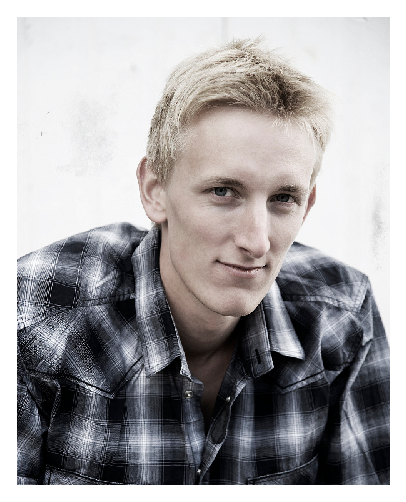
\includegraphics[width=1in,height=1.25in,clip,keepaspectratio]{bio/jo_inge.eps}}]{Jo Inge Buskenes}
received the B.Sc. degree in electrical engineering from Gj\o{}vik College University, Norway, in 2007, and the M.Sc. degree in instrumentation for particle physics from the University of Oslo, Norway, in 2010. He is currently pursuing the Ph.D. degree in acoustic image reconstruction and high performance computing at the University of Oslo.

His industry experience includes development of digital electronics at the European Organization for Nuclear Research (CERN), Geneva, Switzerland (2007-2008). He has lectured in digital signal processing at the Gj\o{}vik College University (2009), and at the University of Oslo (2010-2013). Current affiliation is with The Norwegian Defence Research Establishment, Kjeller, Norway, for which he is developing radar systems (2015-), and formerly sonar systems (2009, 2013).

His research interests include radar and sonar technology, aptive image reconstruction, high performance computing, intelligent detector design and open source software.
\end{IEEEbiography}

\begin{IEEEbiography}[{\includegraphics[width=1in,height=1.25in,clip,keepaspectratio]{bio/roy_color.eps}}]{Roy Edgar Hansen} (M'07) received the M.Sc. and Ph.D. degrees in physics from the University of Troms\o, Troms\o, Norway, in 1992 and 1999, respectively.
The PhD thesis is named Measurements in the Mixed Layer by a Bistatic Multi-CW Doppler Sonar. 
From 1992 to 2000, he was with the Norwegian research company TRIAD, working on multistatic sonar, multistatic radar, synthetic aperture radar (SAR), and underwater communications. Since 2000, he has been with the Norwegian Defence Research Establishment (FFI), Kjeller, Norway. 
In the period 2009-2015, he was research manager for the autonomous underwater vehicle development at FFI, including the fields underwater navigation, battery and fuel-cell technologies, decisional autonomy, and synthetic aperture sonar. 
He is currently principal scientist at FFI. 
He is also adjunct associated professor at Department of informatics at University in Oslo, Norway.
His research interests include synthetic aperture sonar and radar, ultrasound imaging, and array signal processing.
\end{IEEEbiography}

\begin{IEEEbiography}[{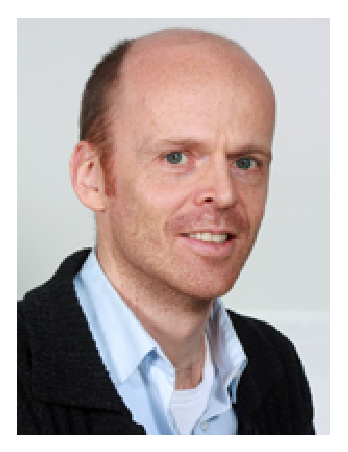
\includegraphics[width=1in,height=1.25in,clip,keepaspectratio]{bio/andreas.eps}}]{Andreas Austeng}
was born in Oslo, Norway, in 1970. He received the M.Sc. degree in physics in 1996 and the Ph.D. degree in computer science in 2001, both from the University of Oslo. Since 2001, he has been working at the Department of Informatics, University of Oslo, first as a postdoctoral research fellow and currently as an associate professor. His research interests include signal and array processing for acoustical imaging.
\end{IEEEbiography}

\vfill 


\end{document}


